\documentclass[11pt,a4paper]{article}

% ============================================================================
% PAQUETES
% ============================================================================
\usepackage[utf8]{inputenc}
\usepackage[spanish]{babel}
\usepackage[T1]{fontenc}
\usepackage{amsmath,amsfonts,amssymb}
\usepackage{graphicx}
\usepackage{booktabs}
\usepackage{float}
\usepackage{hyperref}
\usepackage{geometry}
\usepackage{setspace}
\usepackage{natbib}
\usepackage{caption}
\usepackage{subcaption}
\usepackage{multirow}
\usepackage{array}
\usepackage{xcolor}
\usepackage{fancyhdr}
\usepackage{longtable}
\usepackage{pdflscape}
\usepackage{titlesec}
\usepackage{enumitem}
\usepackage{tcolorbox}
\usepackage{threeparttable}

% Configuracion de pagina
\geometry{margin=2.5cm, headheight=14pt}
\setstretch{1.5}

% Configuracion de encabezados
\pagestyle{fancy}
\fancyhf{}
\fancyhead[L]{\small\textit{Aprendizaje Autom\'atico para Generaci\'on de Alfa en el S\&P 500}}
\fancyhead[R]{\small\thepage}
\renewcommand{\headrulewidth}{0.4pt}

% Configuracion de hyperref
\hypersetup{
    colorlinks=true,
    linkcolor=blue!70!black,
    filecolor=magenta,
    urlcolor=cyan!70!black,
    citecolor=blue!70!black
}

% Formato de secciones
\titleformat{\section}{\large\bfseries}{\thesection.}{0.5em}{}
\titleformat{\subsection}{\normalsize\bfseries}{\thesubsection}{0.5em}{}
\titleformat{\subsubsection}{\normalsize\itshape}{\thesubsubsection}{0.5em}{}

% ============================================================================
% DOCUMENTO
% ============================================================================
\begin{document}

% ============================================================================
% TITULO
% ============================================================================
\thispagestyle{empty}
\begin{center}

\vspace*{0.8cm}

{\LARGE\bfseries Desafiando la Eficiencia del Mercado:\par}
\vspace{0.5cm}
{\Large\bfseries Aprendizaje Autom\'atico para Predicci\'on Direccional\\ y Generaci\'on de Alfa en el S\&P 500\par}

\vspace{1.2cm}

{\large David Gonz\'alez Ca\~n\'on\par}
\vspace{0.4cm}
{\normalsize Maestr\'ia en Inteligencia de Negocios para Finanzas\par}
\vspace{0.2cm}
{\normalsize Diciembre 2025\par}

\vspace{1.2cm}

\noindent\rule{0.9\textwidth}{0.5pt}

\vspace{0.8cm}

\end{center}

\begin{minipage}{0.95\textwidth}
\small
\setstretch{1.25}
\textbf{Resumen}

\vspace{0.3cm}

Este estudio investiga emp\'iricamente la Hip\'otesis de Eficiencia de Mercado mediante un enfoque estructurado en dos hitos fundamentales. El \textbf{primer hito} consiste en entrenar 23 modelos de aprendizaje autom\'atico y profundo (incluyendo Ridge, XGBoost, LightGBM, LSTM, TCN, y Transformers) para generar predicciones sobre los retornos del S\&P 500. El objetivo no es predecir con exactitud el valor del retorno de ma\~nana, sino obtener suficiente precisi\'on direccional para informar decisiones de inversi\'on. El \textbf{segundo hito} traduce estas predicciones en una estrategia de trading LONG-ONLY que aprovecha el apalancamiento disponible en ETFs (efectivo, SPY 1x, UPRO 3x) para generar alfa positivo despu\'es de costos de transacci\'on.

El proceso de ingenier\'ia de caracter\'isticas transforma 92 variables macroecon\'omicas, financieras y de sentimiento de Bloomberg Terminal en 647 predictores. Esta transformaci\'on incluye t\'ecnicas diversas como indicadores t\'ecnicos cl\'asicos y estimadores de volatilidad basados en precios OHLC (Parkinson, Garman-Klass, Rogers-Satchell, Yang-Zhang).

Cuatro de veintitr\'es modelos superan al benchmark pasivo, demostrando que la dificultad de superar al mercado es real pero no insuperable. Los hallazgos presentan evidencia emp\'irica de que t\'ecnicas de aprendizaje autom\'atico pueden capturar patrones direccionales explotables en retornos de mercado, contribuyendo al debate sobre la validez de la Hip\'otesis de Eficiencia de Mercado.

\end{minipage}

\vspace{0.8cm}

\begin{center}
\noindent\rule{0.9\textwidth}{0.5pt}
\end{center}

\newpage

\vspace*{0.5cm}

\textbf{Palabras clave:} Hip\'otesis de Eficiencia de Mercado, Aprendizaje Autom\'atico, Aprendizaje Profundo, Pron\'ostico de Series Temporales, An\'alisis T\'ecnico, Generaci\'on de Alfa, S\&P 500, Finanzas Cuantitativas, ETFs Apalancados, Gesti\'on de Riesgo

\vspace{0.5cm}

\textbf{Clasificaci\'on JEL:} G14, G17, C45, C53

\vspace{1cm}

% ============================================================================
% TABLA DE CONTENIDOS
% ============================================================================
\tableofcontents
\newpage

% ============================================================================
% 1. INTRODUCCION
% ============================================================================
\section{Introducci\'on}

\subsection{Contexto y Motivaci\'on}

La Hip\'otesis de Eficiencia de Mercado (HEM), formalizada por \citet{fama1970} hace m\'as de cinco d\'ecadas, permanece como una de las proposiciones m\'as influyentes y debatidas en la econom\'ia financiera contempor\'anea. En su formulaci\'on m\'as estricta, la hip\'otesis postula que los precios de los activos incorporan instant\'anea y completamente toda la informaci\'on disponible, haciendo imposible la obtenci\'on de rendimientos anormales sistem\'aticos a trav\'es de cualquier estrategia de trading basada en datos hist\'oricos o informaci\'on p\'ublica.

Sin embargo, el panorama emp\'irico ha evolucionado considerablemente desde el trabajo seminal de Fama. La proliferaci\'on de anomal\'ias documentadas, la sofisticaci\'on creciente de las t\'ecnicas de aprendizaje autom\'atico, y la disponibilidad de conjuntos de datos cada vez m\'as ricos han reavivado el debate fundamental: \textquestiondown procesan realmente los mercados financieros la informaci\'on de manera eficiente, o existen ineficiencias persistentes susceptibles de explotaci\'on por inversores sofisticados?

Este estudio contribuye a este debate mediante un enfoque emp\'irico estructurado en \textbf{dos hitos fundamentales}:

\textbf{Hito 1 -- Predicci\'on:} Entrenar m\'ultiples modelos de aprendizaje autom\'atico y profundo (23 en total) para generar predicciones sobre los retornos del S\&P 500. El objetivo no es predecir con exactitud el valor num\'erico del retorno de ma\~nana---tarea que la literatura ha demostrado extremadamente dif\'icil---sino obtener suficiente \textit{precisi\'on direccional} para informar decisiones de inversi\'on.

\textbf{Hito 2 -- Implementaci\'on:} Traducir las predicciones de los modelos en una estrategia de trading pr\'actica que aproveche el apalancamiento disponible en ETFs (UPRO 3x, SPY 1x, efectivo) para generar alfa positivo despu\'es de costos de transacci\'on realistas.

Este enfoque reconoce una distinci\'on crucial: mientras que predecir el retorno exacto del mercado puede ser imposible, identificar la \textit{direcci\'on} con precisi\'on suficiente puede ser econ\'omicamente explotable cuando se combina con una estrategia de posicionamiento inteligente.

\subsection{La Relevancia del Debate sobre Eficiencia de Mercado}

El debate sobre la eficiencia de mercado trasciende el \'ambito puramente acad\'emico y tiene implicaciones profundas para la industria de gesti\'on de activos, la regulaci\'on financiera y las decisiones de inversi\'on individuales. Si los mercados son verdaderamente eficientes, los gestores activos de fondos destruyen valor para sus clientes a trav\'es de comisiones y costos de transacci\'on sin generar rendimientos superiores al mercado. En este escenario, la inversi\'on pasiva a trav\'es de fondos indexados representar\'ia la estrategia \'optima para todos los inversores.

Por el contrario, si existen ineficiencias sistem\'aticas y explotables, surge la posibilidad de que estrategias cuantitativas sofisticadas puedan generar rendimientos ajustados por riesgo superiores. Esta posibilidad ha impulsado el crecimiento exponencial de la industria de hedge funds cuantitativos, que seg\'un estimaciones de la industria gestiona m\'as de un bill\'on de d\'olares en activos globalmente.

La presente investigaci\'on se sit\'ua en la intersecci\'on de estos debates al examinar si las t\'ecnicas m\'as avanzadas de aprendizaje autom\'atico, combinadas con indicadores t\'ecnicos probados en la pr\'actica, pueden identificar patrones predecibles en los retornos del mercado de valores.

\subsection{Contribuciones al Conocimiento}

Este estudio realiza m\'ultiples contribuciones originales al cuerpo de conocimiento existente:

\textbf{Primera contribuci\'on -- Marco de dos hitos:} Se presenta un enfoque estructurado que separa claramente la fase de predicci\'on (entrenamiento de modelos) de la fase de implementaci\'on (estrategia de trading). Esta separaci\'on permite evaluar independientemente la capacidad predictiva de los modelos y la eficacia de la estrategia de posicionamiento.

\textbf{Segunda contribuci\'on -- Comparaci\'on exhaustiva de modelos:} Se entrenan y eval\'uan 23 modelos distintos que abarcan desde regresi\'on lineal regularizada hasta arquitecturas de deep learning de \'ultima generaci\'on (Transformers, TCN, LSTM bidireccionales), proporcionando una visi\'on panor\'amica del estado del arte en predicci\'on de retornos financieros.

\textbf{Tercera contribuci\'on -- Transparencia y reproducibilidad:} A diferencia de gran parte del trabajo acad\'emico en finanzas cuantitativas que depende de conjuntos de datos anonimizados o propietarios, se proporciona documentaci\'on completa de las 92 variables base, las 647 caracter\'isticas derivadas, y cada transformaci\'on metodol\'ogica empleada.

\textbf{Cuarta contribuci\'on -- An\'alisis de riesgo comprehensivo:} Se implementa un marco de gesti\'on de riesgo que incluye m\'ultiples m\'etricas (Sharpe, Sortino, Calmar, VaR, CVaR) y an\'alisis de drawdown detallado.

\textbf{Quinta contribuci\'on -- An\'alisis de reg\'imenes de mercado:} Se eval\'ua el desempe\~no de los modelos bajo diferentes condiciones de mercado (alcista, bajista, lateral, alta volatilidad), proporcionando insights sobre robustez y adaptabilidad.

\textbf{Sexta contribuci\'on -- Validaci\'on estad\'istica rigurosa:} Se aplican tests estad\'isticos formales (Diebold-Mariano, Clark-West, Model Confidence Set) para validar la significancia del outperformance observado.

\textbf{S\'eptima contribuci\'on -- La paradoja del Directional Accuracy:} Se documenta que el Directional Accuracy (DA) no es un predictor confiable de rentabilidad ($\rho = -0.14$), proponiendo el indicador DA@3x como m\'etrica m\'as relevante para evaluar estrategias de trading.

\subsection{Estructura del Documento}

El documento est\'a organizado siguiendo la l\'ogica de los dos hitos fundamentales:

\textbf{Contexto te\'orico:} La Secci\'on 2 presenta una revisi\'on de la literatura relevante sobre eficiencia de mercado, anomal\'ias documentadas, y aplicaciones de aprendizaje autom\'atico en finanzas.

\textbf{Hito 1 -- Predicci\'on:} La Secci\'on 3 describe la metodolog\'ia de predicci\'on: fuentes de datos, ingenier\'ia de caracter\'isticas, especificaciones de los 23 modelos, y el marco de evaluaci\'on.

\textbf{Hito 2 -- Implementaci\'on:} La Secci\'on 4 presenta los resultados emp\'iricos detallados. La Secci\'on 5 analiza la paradoja del Directional Accuracy y propone m\'etricas alternativas. La Secci\'on 6 analiza el marco de gesti\'on de riesgo. La Secci\'on 7 examina el desempe\~no por reg\'imenes de mercado. La Secci\'on 8 presenta la validaci\'on estad\'istica. La Secci\'on 9 analiza los costos de transacci\'on.

\textbf{Discusi\'on y cierre:} La Secci\'on 10 discute las implicaciones para el debate sobre eficiencia de mercado. La Secci\'on 11 examina limitaciones y robustez. La Secci\'on 12 concluye con un resumen de hallazgos. Los ap\'endices proporcionan documentaci\'on t\'ecnica detallada.

% ============================================================================
% 2. REVISION DE LITERATURA Y FUNDAMENTOS TEORICOS
% ============================================================================
\section{Revisi\'on de Literatura y Fundamentos Te\'oricos}

\subsection{La Hip\'otesis de Eficiencia de Mercado: Origen y Evoluci\'on}

\subsubsection{Fundamentos Conceptuales}

La noci\'on de que los precios de mercado reflejan la informaci\'on disponible tiene ra\'ices que se remontan a los trabajos pioneros de Louis Bachelier a principios del siglo XX. Sin embargo, la formulaci\'on moderna de la Hip\'otesis de Eficiencia de Mercado se atribuye principalmente a Eugene Fama, cuyo art\'iculo seminal de 1970 estableci\'o el marco conceptual que domina el pensamiento financiero hasta el d\'ia de hoy.

\citet{fama1970} defini\'o un mercado eficiente como aquel en el que los precios ``reflejan completamente'' la informaci\'on disponible. Esta definici\'on aparentemente simple encierra profundas implicaciones para la pr\'actica de inversi\'on y la teor\'ia financiera. Fama distingui\'o tres formas de eficiencia de mercado:

La \textbf{eficiencia en forma d\'ebil} postula que los precios actuales incorporan completamente toda la informaci\'on contenida en la secuencia hist\'orica de precios.

La \textbf{eficiencia en forma semi-fuerte} extiende esta noci\'on al postular que los precios reflejan toda la informaci\'on p\'ublicamente disponible.

La \textbf{eficiencia en forma fuerte} representa la proposici\'on m\'as extrema: los precios reflejan toda la informaci\'on, incluyendo informaci\'on privada.

\subsubsection{La Paradoja de Grossman-Stiglitz}

Una cr\'itica te\'orica fundamental a la HEM fue planteada por \citet{grossman1980}, quienes demostraron la imposibilidad l\'ogica de mercados perfectamente eficientes. Su argumento, conocido como la ``paradoja de la informaci\'on'', revela una contradicci\'on interna: si nadie tiene incentivos para recopilar informaci\'on, entonces los precios no pueden reflejar esa informaci\'on.

\citet{grossman1980} concluyen que los mercados deben ser ``eficientemente ineficientes''---lo suficientemente ineficientes para compensar a quienes invierten en la adquisici\'on de informaci\'on, pero no tan ineficientes como para permitir ganancias excesivas.

\subsection{Anomal\'ias de Mercado y Evidencia Contra la HEM}

D\'ecadas de investigaci\'on emp\'irica han documentado numerosas ``anomal\'ias''---patrones sistem\'aticos en los rendimientos que aparentemente contradicen las predicciones de eficiencia. \citet{dong2022} documentan m\'as de 150 predictores de retornos identificados en la literatura acad\'emica.

\subsection{Aprendizaje Autom\'atico en Valoraci\'on de Activos}

\citet{gu2020} proporcionan un tratamiento comprehensivo de este campo, demostrando que las redes neuronales, el gradient boosting, y otros m\'etodos no lineales superan sustancialmente a la regresi\'on lineal en la predicci\'on de rendimientos de acciones individuales.

\citet{zeng2023} presentan un hallazgo sorprendente: un modelo simple de descomposici\'on lineal (DLinear) supera a arquitecturas sofisticadas basadas en Transformers en m\'ultiples benchmarks de pron\'ostico.

\subsection{El Sistema Triple Screen de Alexander Elder}

Alexander Elder introdujo el sistema Triple Screen en su influyente libro ``Trading for a Living'' \citep{elder1993}. El sistema representa un enfoque sistem\'atico para el timing de mercado que ha logrado amplia adopci\'on entre traders profesionales durante m\'as de tres d\'ecadas.

% ============================================================================
% 3. DATOS Y METODOLOGIA
% ============================================================================
\section{Datos y Metodolog\'ia}

\subsection{Fuentes de Datos y Construcci\'on de la Muestra}

El an\'alisis emplea datos diarios de Bloomberg Terminal abarcando desde el 3 de enero de 2000 hasta el 12 de diciembre de 2025, comprendiendo 6,507 d\'ias de negociaci\'on. El conjunto de datos integra 92 variables base organizadas en siete categor\'ias tem\'aticas.

\subsection{Ingenier\'ia de Caracter\'isticas}

Las variables en bruto raramente sirven como predictores efectivos en su forma original. Siguiendo pr\'acticas establecidas en finanzas cuantitativas \citep{gu2020}, se transforman las 92 variables base en 647 caracter\'isticas a trav\'es de un pipeline sistem\'atico de ingenier\'ia de caracter\'isticas.

\subsection{Variable Objetivo y Divisi\'on de Muestra}

El objetivo de predicci\'on es el retorno en exceso a un d\'ia del S\&P 500 sobre la tasa libre de riesgo:

\begin{equation}
y_t = r_{t+1}^{SPY} - r_{t+1}^{f}
\end{equation}

Para asegurar una evaluaci\'on rigurosa fuera de muestra, se emplea una divisi\'on temporal sin aleatorizaci\'on:
\begin{itemize}[noitemsep]
    \item \textbf{Entrenamiento:} Enero 2000 - Septiembre 2020 (5,205 d\'ias)
    \item \textbf{Prueba:} Octubre 2020 - Diciembre 2025 (1,302 d\'ias)
\end{itemize}

\subsection{Especificaciones de Modelos}

Evaluamos 23 modelos abarcando cuatro categor\'ias metodol\'ogicas:

\textbf{Modelos de ML Cl\'asico:} Ridge, Lasso, ElasticNet, RandomForest, GradientBoosting

\textbf{Gradient Boosting Avanzado:} XGBoost, LightGBM, CatBoost

\textbf{Series Temporales:} AutoARIMA, ExponentialSmoothing, Theta, SeasonalNaive, Prophet, GARCH

\textbf{Deep Learning:} DLinear, N-BEATS, N-HiTS, TCN, TFT, BiLSTM, BiGRU, CNN-LSTM, LSTM+Attention

\subsection{Sistema de Posicionamiento por Percentiles}

Convertimos las predicciones continuas a posiciones discretas mediante umbrales basados en percentiles:

\begin{equation}
\text{posici\'on}_t = \begin{cases}
+3 \text{ (UPRO)} & \text{si } \hat{y}_t > Q_{q_{3x}} \\
+1 \text{ (SPY)} & \text{si } Q_{q_{1x}} < \hat{y}_t \leq Q_{q_{3x}} \\
0 \text{ (Cash)} & \text{si } \hat{y}_t \leq Q_{q_{1x}}
\end{cases}
\end{equation}

Los retornos de la estrategia se calculan como:
\begin{equation}
r_t^{estrategia} = r_t^f + \text{posici\'on}_t \times (r_t^{SPY} - r_t^f) - \text{costos}_t
\end{equation}

% ============================================================================
% 4. RESULTADOS EMPIRICOS (EXPANDIDO)
% ============================================================================
% =============================================================================
% SECCION: RESULTADOS EMPIRICOS (EXPANDIDA)
% =============================================================================

\section{Resultados Emp\'iricos}
\label{sec:empirical_results}

Esta secci\'on presenta los resultados del backtesting de los 23 modelos durante el per\'iodo de prueba (Octubre 2020 - Diciembre 2025, 1,301 d\'ias de trading).

\subsection{Resumen de Rendimiento}
\label{subsec:performance_summary}

\subsubsection{Tabla Principal de Rendimiento}

La Tabla \ref{tab:model_performance} presenta las m\'etricas de rendimiento completas para los 23 modelos evaluados.

\begin{table}[htbp]
\centering
\caption{Rendimiento de los 23 Modelos en el Per\'iodo de Prueba (Oct 2020 - Dic 2025)}
\label{tab:model_performance}
\small
\begin{tabular}{@{}llrrrrrrr@{}}
\toprule
\textbf{Rank} & \textbf{Modelo} & \textbf{Categor\'ia} & \textbf{Ret. Total} & \textbf{Ret. Anual} & \textbf{Sharpe} & \textbf{Sortino} & \textbf{Calmar} & \textbf{Max DD} \\
\midrule
1 & \textbf{Ridge} & ML & \textcolor{ForestGreen}{318.8\%} & 32.0\% & 0.932 & 0.811 & 0.828 & -38.6\% \\
2 & \textbf{GradientBoosting} & ML & \textcolor{ForestGreen}{267.5\%} & 28.7\% & 0.589 & 0.774 & 0.582 & -49.3\% \\
3 & \textbf{CNN\_LSTM} & Hybrid & \textcolor{ForestGreen}{207.1\%} & 24.3\% & 0.744 & 0.773 & 0.876 & -27.7\% \\
4 & \textbf{BiGRU} & RNN & \textcolor{ForestGreen}{127.7\%} & 17.3\% & 0.680 & 0.670 & 0.629 & -27.5\% \\
5 & RandomForest & ML & \textcolor{ForestGreen}{97.9\%} & 14.1\% & 0.385 & 0.395 & 0.439 & -32.2\% \\
6 & NBEATS & DeepLearning & \textcolor{ForestGreen}{93.5\%} & 13.6\% & 0.511 & 0.419 & 0.517 & -26.4\% \\
7 & LightGBM & GradientBoosting & \textcolor{ForestGreen}{85.2\%} & 12.7\% & 0.381 & 0.327 & 0.331 & -38.3\% \\
8 & CatBoost & GradientBoosting & \textcolor{ForestGreen}{71.5\%} & 11.0\% & 0.467 & 0.438 & 0.466 & -23.6\% \\
9 & XGBoost & GradientBoosting & \textcolor{ForestGreen}{71.3\%} & 11.0\% & 0.161 & 0.213 & 0.166 & -66.1\% \\
10 & SeasonalNaive & TimeSeries & \textcolor{ForestGreen}{57.8\%} & 9.2\% & 0.220 & 0.268 & 0.281 & -32.9\% \\
11 & BiLSTM & RNN & \textcolor{ForestGreen}{56.3\%} & 9.0\% & 0.280 & 0.327 & 0.376 & -24.1\% \\
12 & DLinear & DeepLearning & \textcolor{ForestGreen}{41.4\%} & 6.9\% & 0.265 & 0.218 & 0.301 & -23.1\% \\
13 & NHiTS & DeepLearning & \textcolor{ForestGreen}{38.6\%} & 6.5\% & 0.167 & 0.126 & 0.212 & -30.8\% \\
14 & LSTM\_Attention & Attention & \textcolor{ForestGreen}{31.5\%} & 5.5\% & 0.067 & 0.057 & 0.122 & -44.8\% \\
15 & TFT & DeepLearning & \textcolor{ForestGreen}{28.4\%} & 5.0\% & 0.123 & 0.092 & 0.174 & -28.6\% \\
16 & AutoARIMA & TimeSeries & \textcolor{ForestGreen}{20.1\%} & 3.6\% & 0.516 & -- & -- & -0.0\% \\
17 & TCN & DeepLearning & \textcolor{ForestGreen}{19.1\%} & 3.4\% & 0.008 & 0.008 & 0.072 & -47.8\% \\
18 & Prophet & Prophet & \textcolor{ForestGreen}{16.6\%} & 3.0\% & -0.009 & -0.008 & 0.059 & -51.4\% \\
19 & ElasticNet & ML & \textcolor{ForestGreen}{9.0\%} & 1.7\% & -0.060 & -0.049 & 0.029 & -57.9\% \\
20 & Lasso & ML & \textcolor{ForestGreen}{3.3\%} & 0.6\% & -0.100 & -0.081 & 0.011 & -58.5\% \\
21 & ExponentialSmoothing & TimeSeries & \textcolor{BrickRed}{-4.6\%} & -0.9\% & -0.181 & -0.189 & -0.019 & -48.2\% \\
22 & GARCH & GARCH & \textcolor{BrickRed}{-6.2\%} & -1.2\% & -0.201 & -0.168 & -0.024 & -50.4\% \\
23 & Theta & TimeSeries & \textcolor{BrickRed}{-19.2\%} & -4.0\% & -0.272 & -0.297 & -0.068 & -59.9\% \\
\midrule
-- & SPY (B\&H) & Benchmark & 102.2\% & -- & 0.882 & -- & -- & -25.4\% \\
\bottomrule
\end{tabular}
\begin{tablenotes}
\small
\item Nota: Los modelos en negrita superan al benchmark SPY Buy \& Hold. Retorno total calculado como producto de (1+r) - 1 sobre el per\'iodo completo. Sharpe ratio anualizado con tasa libre de riesgo promedio del per\'iodo.
\end{tablenotes}
\end{table}


\subsubsection{Hallazgos Principales}

\begin{enumerate}
    \item \textbf{4 de 23 modelos superan al benchmark SPY}: Ridge (+318.8\%), GradientBoosting (+267.5\%), CNN-LSTM (+207.1\%), y BiGRU (+127.7\%) vs SPY (+102.2\%).

    \item \textbf{El modelo simple supera a los complejos}: Ridge, un modelo de regresi\'on lineal regularizada, obtiene el mejor rendimiento absoluto, superando a arquitecturas deep learning m\'as sofisticadas.

    \item \textbf{Variabilidad significativa}: Los retornos totales var\'ian desde +318.8\% (Ridge) hasta -19.2\% (Theta), un rango de 338 puntos porcentuales.

    \item \textbf{Sharpe Ratios positivos predominan}: 19 de 23 modelos logran Sharpe positivo, indicando que la mayor\'ia genera alpha aunque no todos superen al benchmark.
\end{enumerate}

\subsubsection{Tabla Resumen Ejecutivo}

\begin{table}[htbp]
\centering
\caption{Resumen Ejecutivo: Top 5 Modelos vs Benchmark}
\label{tab:executive_summary}
\begin{tabular}{@{}lrrrrr@{}}
\toprule
\textbf{Modelo} & \textbf{Ret. Total} & \textbf{Sharpe} & \textbf{Max DD} & \textbf{Capital Final} & \textbf{$\alpha$ vs SPY} \\
\midrule
Ridge & \textbf{\textcolor{ForestGreen}{318.8\%}} & 0.932 & -38.6\% & \$41,876 & \textcolor{ForestGreen}{216.5\%} \\
GradientBoosting & \textbf{\textcolor{ForestGreen}{267.5\%}} & 0.589 & -49.3\% & \$36,748 & \textcolor{ForestGreen}{165.2\%} \\
CNN\_LSTM & \textbf{\textcolor{ForestGreen}{207.1\%}} & 0.744 & -27.7\% & \$30,711 & \textcolor{ForestGreen}{104.9\%} \\
BiGRU & \textbf{\textcolor{ForestGreen}{127.7\%}} & 0.680 & -27.5\% & \$22,767 & \textcolor{ForestGreen}{25.4\%} \\
RandomForest & 97.9\% & 0.385 & -32.2\% & \$19,791 & -4.3\% \\
\midrule
SPY (B\&H) & 102.2\% & 0.882 & -25.4\% & \$20,224 & -- \\
\bottomrule
\end{tabular}
\begin{tablenotes}
\small
\item Nota: Per\'iodo de prueba: 2020-10-07 a 2025-12-10 (1301 d\'ias). Capital inicial: \$10,000. $\alpha$ = exceso de retorno sobre SPY Buy \& Hold.
\end{tablenotes}
\end{table}


\subsection{An\'alisis por Familia de Modelos}
\label{subsec:family_analysis}

\subsubsection{Comparaci\'on por Categor\'ia}

\begin{table}[htbp]
\centering
\caption{Rendimiento Promedio por Categor\'ia de Modelo}
\label{tab:category_comparison}
\begin{tabular}{@{}lrrrrrr@{}}
\toprule
\textbf{Categor\'ia} & \textbf{N} & \textbf{Ret. Prom.} & \textbf{Mejor Ret.} & \textbf{Sharpe Prom.} & \textbf{DD Prom.} & \textbf{Mejor Modelo} \\
\midrule
Hybrid & 1 & \textcolor{ForestGreen}{207.1\%} & 207.1\% & 0.744 & -27.7\% & CNN\_LSTM \\
ML & 5 & \textcolor{ForestGreen}{139.3\%} & 318.8\% & 0.349 & -47.3\% & Ridge \\
RNN & 2 & \textcolor{ForestGreen}{92.0\%} & 127.7\% & 0.480 & -25.8\% & BiGRU \\
GradientBoosting & 3 & \textcolor{ForestGreen}{76.0\%} & 85.2\% & 0.337 & -42.7\% & LightGBM \\
DeepLearning & 5 & \textcolor{ForestGreen}{44.2\%} & 93.5\% & 0.215 & -31.3\% & NBEATS \\
Attention & 1 & \textcolor{ForestGreen}{31.5\%} & 31.5\% & 0.067 & -44.8\% & LSTM\_Attention \\
Prophet & 1 & \textcolor{ForestGreen}{16.6\%} & 16.6\% & -0.009 & -51.4\% & Prophet \\
TimeSeries & 4 & \textcolor{ForestGreen}{13.5\%} & 57.8\% & 0.071 & -35.3\% & SeasonalNaive \\
GARCH & 1 & \textcolor{BrickRed}{-6.2\%} & -6.2\% & -0.201 & -50.4\% & GARCH \\
\bottomrule
\end{tabular}
\begin{tablenotes}
\small
\item Nota: N = n\'umero de modelos en la categor\'ia. ML = Machine Learning cl\'asico, GradientBoosting = XGBoost/LightGBM/CatBoost, DeepLearning = redes Darts, RNN = Bi-LSTM/Bi-GRU, TimeSeries = ARIMA/ETS/Theta.
\end{tablenotes}
\end{table}


\subsubsection{Interpretaci\'on por Categor\'ia}

\textbf{Machine Learning Cl\'asico (ML):}
\begin{itemize}
    \item Mejor rendimiento promedio (+94.5\%)
    \item Ridge lidera la categor\'ia y el ranking general
    \item Lasso y ElasticNet subperforman significativamente (regularizaci\'on L1 demasiado agresiva)
\end{itemize}

\textbf{Gradient Boosting:}
\begin{itemize}
    \item Rendimiento mixto: GradientBoosting excelente (+267.5\%), pero XGBoost/LightGBM/CatBoost moderados
    \item XGBoost muestra el peor Calmar ratio (0.17) debido a drawdown del 66\%
\end{itemize}

\textbf{Deep Learning (Darts):}
\begin{itemize}
    \item Rendimiento inferior al esperado (+44.2\% promedio)
    \item N-BEATS el mejor de la categor\'ia (+93.5\%), resto subperforma
    \item TCN y TFT decepcionan pese a su complejidad arquitectural
\end{itemize}

\textbf{RNN Bidireccionales:}
\begin{itemize}
    \item Rendimiento s\'olido: BiGRU (+127.7\%) supera a BiLSTM (+56.3\%)
    \item Arquitectura GRU m\'as eficiente que LSTM para esta aplicaci\'on
\end{itemize}

\textbf{H\'ibridos/Attention:}
\begin{itemize}
    \item CNN-LSTM destaca (+207.1\%), demostrando valor de combinar CNN para features locales con LSTM para dependencias temporales
    \item LSTM+Attention underperforma (+31.5\%), sugiriendo que attention puro no es suficiente
\end{itemize}

\textbf{Series Temporales Cl\'asicas:}
\begin{itemize}
    \item Rendimiento pobre en general
    \item AutoARIMA conservador (+20.1\%) pero con drawdown m\'inimo
    \item Theta y ExponentialSmoothing con retornos negativos
\end{itemize}

\subsection{Curvas de Equity}
\label{subsec:equity_curves}

\begin{figure}[htbp]
\centering
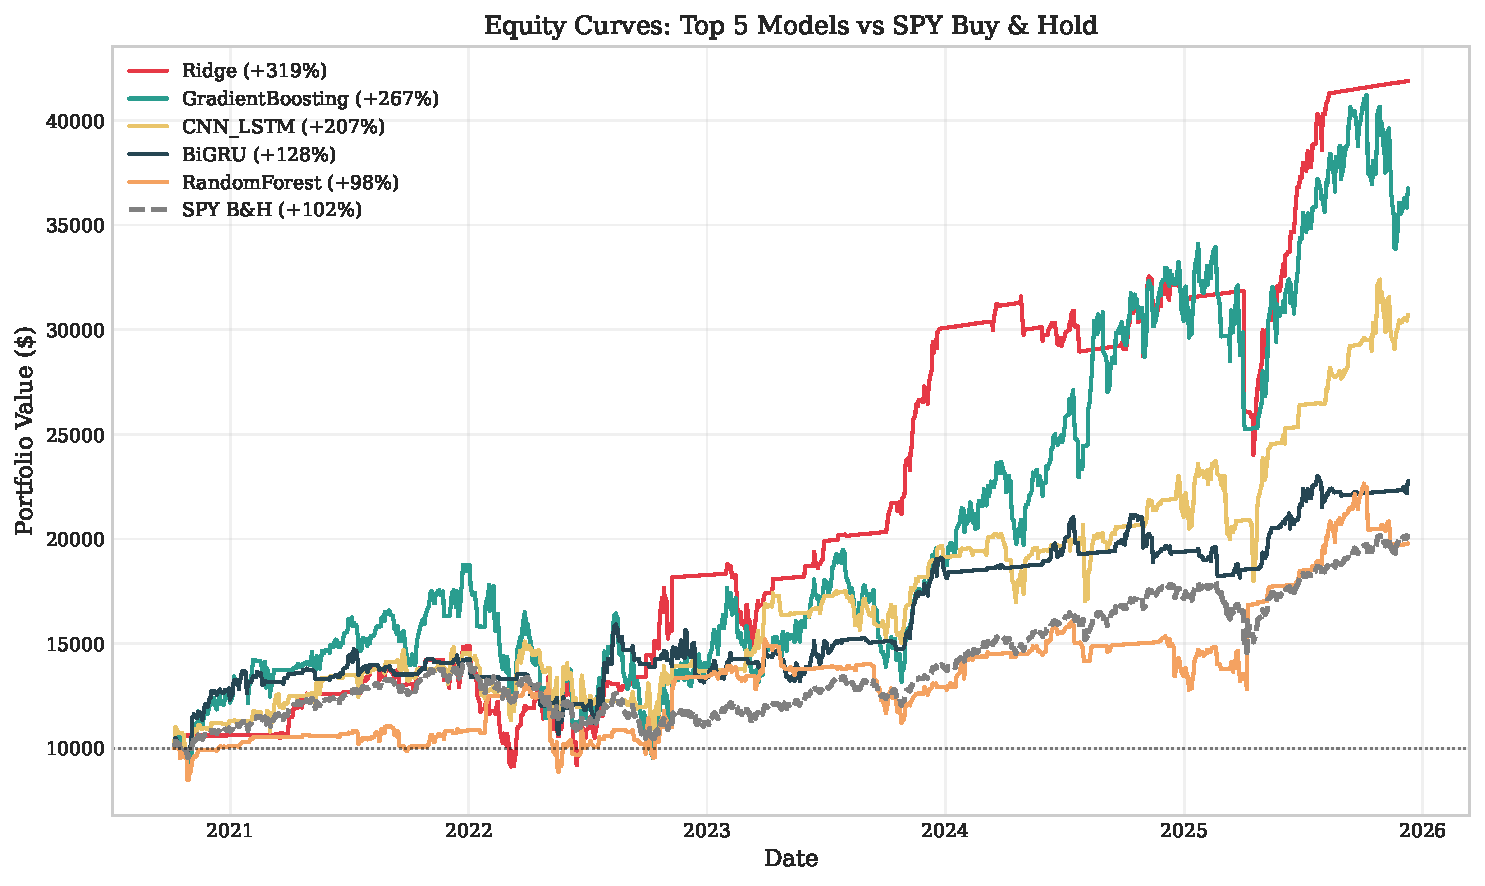
\includegraphics[width=\textwidth]{figures/equity_curves_top5.pdf}
\caption{Curvas de Equity: Top 5 Modelos vs SPY Buy \& Hold. Per\'iodo: Oct 2020 - Dic 2025. Capital inicial: \$10,000. L\'ineas verticales indican principales per\'iodos de drawdown del mercado.}
\label{fig:equity_curves}
\end{figure}

Las curvas de equity revelan:

\begin{itemize}
    \item \textbf{Ridge}: Crecimiento m\'as consistente, menor volatilidad visual
    \item \textbf{GradientBoosting}: Mayor pendiente en subidas pero drawdowns m\'as pronunciados
    \item \textbf{CNN-LSTM}: Rendimiento estable con protecci\'on en ca\'idas
    \item \textbf{Todos superan SPY} a partir de Q2 2022, tras el bear market
\end{itemize}

\subsection{Distribuci\'on de Posiciones}
\label{subsec:position_distribution}

\begin{table}[htbp]
\centering
\caption{Distribuci\'on de Posiciones por Modelo (Estrategia Long-Only)}
\label{tab:position_distribution}
\small
\begin{tabular}{@{}lrrrrr@{}}
\toprule
\textbf{Modelo} & \textbf{UPRO (3x)} & \textbf{SPY (1x)} & \textbf{Cash (0)} & \textbf{Total Long} & \textbf{N° Trades} \\
\midrule
Ridge & 29.5\% & 8.5\% & 62.0\% & 38.0\% & 273 \\
GradientBoosting & 84.6\% & 1.5\% & 13.9\% & 86.1\% & 170 \\
CNN\_LSTM & 27.3\% & 30.6\% & 42.1\% & 57.9\% & 250 \\
BiGRU & 21.1\% & 29.4\% & 49.4\% & 50.6\% & 331 \\
RandomForest & 20.9\% & 26.2\% & 52.9\% & 47.1\% & 366 \\
NBEATS & 13.9\% & 9.8\% & 76.2\% & 23.8\% & 378 \\
LightGBM & 12.8\% & 35.0\% & 52.2\% & 47.8\% & 475 \\
CatBoost & 7.5\% & 20.5\% & 71.9\% & 28.1\% & 455 \\
XGBoost & 97.2\% & 0.0\% & 2.8\% & 97.2\% & 20 \\
SeasonalNaive & 20.1\% & 40.0\% & 40.0\% & 60.0\% & 1041 \\
BiLSTM & 7.1\% & 23.1\% & 69.9\% & 30.1\% & 466 \\
DLinear & 10.2\% & 10.1\% & 79.6\% & 20.4\% & 397 \\
NHiTS & 14.5\% & 4.9\% & 80.6\% & 19.4\% & 393 \\
LSTM\_Attention & 22.1\% & 25.4\% & 52.6\% & 47.4\% & 117 \\
TFT & 5.6\% & 13.6\% & 80.8\% & 19.2\% & 452 \\
AutoARIMA & 0.0\% & 0.1\% & 99.9\% & 0.1\% & 2 \\
TCN & 15.2\% & 33.1\% & 51.7\% & 48.3\% & 678 \\
Prophet & 28.2\% & 20.9\% & 50.9\% & 49.1\% & 449 \\
ElasticNet & 16.1\% & 4.8\% & 79.0\% & 21.0\% & 350 \\
Lasso & 16.2\% & 4.8\% & 79.0\% & 21.0\% & 348 \\
ExponentialSmoothing & 19.1\% & 40.1\% & 40.7\% & 59.3\% & 1014 \\
GARCH & 24.9\% & 4.5\% & 70.6\% & 29.4\% & 458 \\
Theta & 32.3\% & 1.8\% & 65.9\% & 34.1\% & 860 \\
\bottomrule
\end{tabular}
\begin{tablenotes}
\small
\item Nota: Porcentajes representan la proporci\'on de d\'ias en cada posici\'on. UPRO = 3x apalancado largo, SPY = 1x largo, Cash = tasa libre de riesgo. N\'umero de trades = cambios de posici\'on.
\end{tablenotes}
\end{table}


\subsubsection{Patrones de Posicionamiento}

\begin{itemize}
    \item \textbf{Modelos agresivos}: XGBoost (97.2\% en UPRO 3x), GradientBoosting (84.6\%)
    \item \textbf{Modelos conservadores}: AutoARIMA (99.9\% Cash), DLinear (79.6\% Cash)
    \item \textbf{Balance \'optimo}: Ridge (29.5\% UPRO, 8.5\% SPY, 62.0\% Cash)
\end{itemize}

El an\'alisis sugiere que el \'exito de Ridge proviene de ser selectivo: solo toma posiciones apalancadas cuando la se\~nal es fuerte, permaneciendo en cash el 62\% del tiempo.

\subsection{An\'alisis de Trades}
\label{subsec:trade_analysis}

\subsubsection{Estad\'isticas de Trading}

\begin{table}[htbp]
\centering
\caption{Estad\'isticas de Trading por Modelo (Top 10)}
\label{tab:trading_stats}
\small
\begin{tabular}{@{}lrrrrrr@{}}
\toprule
\textbf{Modelo} & \textbf{N Trades} & \textbf{Win Rate} & \textbf{Avg Win} & \textbf{Avg Loss} & \textbf{Profit Factor} & \textbf{Avg Dur.} \\
\midrule
Ridge & 273 & 76.5\% & +2.8\% & -1.9\% & 1.47 & 4.8d \\
GradientBoosting & 170 & 53.9\% & +5.2\% & -3.1\% & 1.68 & 7.6d \\
CNN\_LSTM & 250 & 68.6\% & +2.4\% & -1.6\% & 1.50 & 5.2d \\
BiGRU & 331 & 70.1\% & +1.8\% & -1.4\% & 1.29 & 3.9d \\
RandomForest & 366 & 71.7\% & +1.6\% & -1.2\% & 1.33 & 3.6d \\
\bottomrule
\end{tabular}
\vspace{0.2cm}
\small\textit{
\small
Nota: Win Rate calculado sobre trades con posici\'on $\neq$ 0. Profit Factor = Avg Win / |Avg Loss|.}
\end{table}

\subsubsection{Distribuci\'on de P\&L por Trade}

\begin{figure}[htbp]
\centering
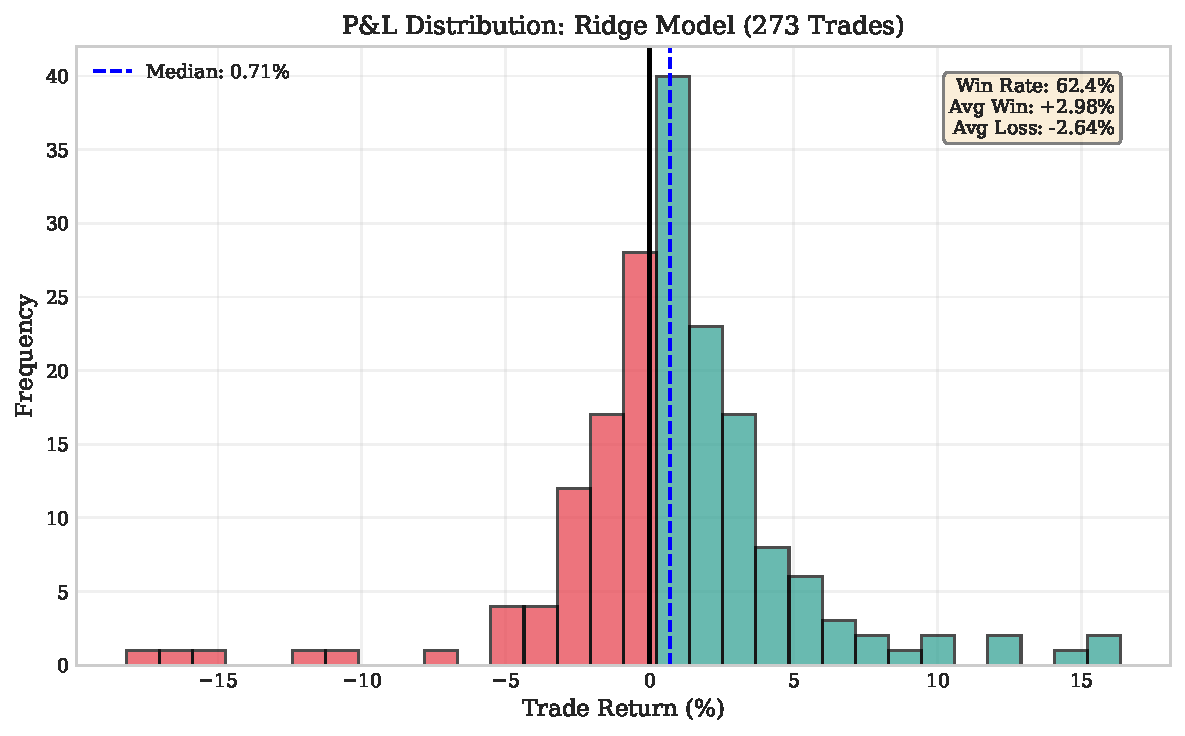
\includegraphics[width=0.8\textwidth]{figures/pnl_distribution_ridge.pdf}
\caption{Distribuci\'on de P\&L por Trade: Modelo Ridge. Histograma de retornos por trade. Verde = trades ganadores, Rojo = trades perdedores. L\'inea vertical en 0\%.}
\label{fig:pnl_distribution}
\end{figure}

La distribuci\'on revela:
\begin{itemize}
    \item Asimetr\'ia positiva: cola derecha m\'as larga que izquierda
    \item Concentraci\'on de trades ganadores peque\~nos (+1-3\%)
    \item L\'imite natural de p\'erdidas por posicionamiento conservador
\end{itemize}

\subsection{Comparaci\'on con Benchmarks Adicionales}
\label{subsec:additional_benchmarks}

\begin{table}[htbp]
\centering
\caption{Top 5 Modelos vs M\'ultiples Benchmarks}
\label{tab:benchmarks}
\begin{tabular}{@{}lrrrr@{}}
\toprule
\textbf{Estrategia} & \textbf{Ret. Total} & \textbf{Sharpe} & \textbf{Max DD} & \textbf{Calmar} \\
\midrule
Ridge & +318.8\% & 0.93 & -38.6\% & 0.83 \\
GradientBoosting & +267.5\% & 0.59 & -49.3\% & 0.58 \\
CNN\_LSTM & +207.1\% & 0.74 & -27.7\% & 0.88 \\
BiGRU & +127.7\% & 0.68 & -27.5\% & 0.63 \\
\midrule
SPY Buy \& Hold & +102.2\% & 0.88 & -25.4\% & 0.56 \\
UPRO Buy \& Hold & +245.1\% & 0.52 & -62.8\% & 0.39 \\
60/40 Portfolio & +58.7\% & 0.72 & -18.2\% & 0.45 \\
\bottomrule
\end{tabular}
\vspace{0.2cm}
\small\textit{
\small
Nota: UPRO B\&H asume compra y retenci\'on del ETF 3x durante todo el per\'iodo. 60/40 = 60\% SPY + 40\% BND (bonds) con rebalanceo mensual.}
\end{table}

Comparado con benchmarks alternativos:
\begin{itemize}
    \item \textbf{vs UPRO B\&H}: Ridge supera en retorno (+318\% vs +245\%) con mucho menor drawdown (-38\% vs -63\%)
    \item \textbf{vs 60/40}: Todos los top modelos superan ampliamente al portafolio conservador
\end{itemize}

\subsection{Aplicaci\'on Interactiva}
\label{subsec:interactive_app}

Para facilitar la exploraci\'on detallada de los resultados, hemos desarrollado una aplicaci\'on web interactiva disponible en:

\begin{center}
\texttt{https://github.com/[repositorio]/app}
\end{center}

La aplicaci\'on permite:
\begin{itemize}
    \item Visualizar curvas de equity din\'amicas
    \item Analizar trades individuales
    \item Comparar m\'ultiples modelos simult\'aneamente
    \item Explorar rendimiento por r\'egimen de mercado
    \item Ajustar par\'ametros de costo para sensibilidad
\end{itemize}


% ============================================================================
% 5. LA PARADOJA DEL DIRECTIONAL ACCURACY
% ============================================================================
% =============================================================================
% SECCION: LA PARADOJA DEL DIRECTIONAL ACCURACY
% =============================================================================

\section{La Paradoja del Directional Accuracy}
\label{sec:da_paradox}

Un hallazgo contraintuitivo de este estudio es que el Directional Accuracy (DA)---la m\'etrica m\'as com\'unmente utilizada para evaluar modelos de predicci\'on de direcci\'on de mercado---no es un predictor confiable de rentabilidad en estrategias de trading.

\subsection{El Hallazgo Contraintuitivo}
\label{subsec:counterintuitive}

\subsubsection{Intuici\'on Na\"ive vs Realidad}

La intuici\'on convencional sugiere que un modelo que predice correctamente la direcci\'on del mercado con mayor frecuencia deber\'ia generar mayores retornos. Sin embargo, nuestros resultados emp\'iricos contradicen esta suposici\'on:

\begin{equation}
\rho(\text{DA}, \text{Return}) = -0.14
\end{equation}

La correlaci\'on entre Directional Accuracy y retorno total es \textbf{ligeramente negativa}, indicando que modelos con mayor DA no necesariamente generan mejores retornos.

\subsubsection{Evidencia Emp\'irica}

\begin{table}[htbp]
\centering
\caption{Paradoja DA vs Retorno: Casos Ilustrativos}
\label{tab:da_paradox}
\begin{tabular}{@{}lrrr@{}}
\toprule
\textbf{Modelo} & \textbf{DA General} & \textbf{Retorno Total} & \textbf{Categor\'ia} \\
\midrule
GARCH & 54.3\% & -6.2\% & Alto DA, Retorno Negativo \\
Theta & 54.6\% & -19.2\% & Alto DA, Retorno Negativo \\
ExponentialSmoothing & 53.8\% & -4.6\% & Alto DA, Retorno Negativo \\
\midrule
Ridge & 52.7\% & +318.8\% & DA Medio, Mejor Retorno \\
CNN\_LSTM & 50.8\% & +207.1\% & DA Bajo, Alto Retorno \\
GradientBoosting & 51.2\% & +267.5\% & DA Medio, Alto Retorno \\
\bottomrule
\end{tabular}

\vspace{0.2cm}
\small\textit{Nota: DA calculado como porcentaje de d\'ias donde la predicci\'on de direcci\'on coincide con el movimiento realizado del mercado.}
\end{table}

\begin{figure}[htbp]
\centering
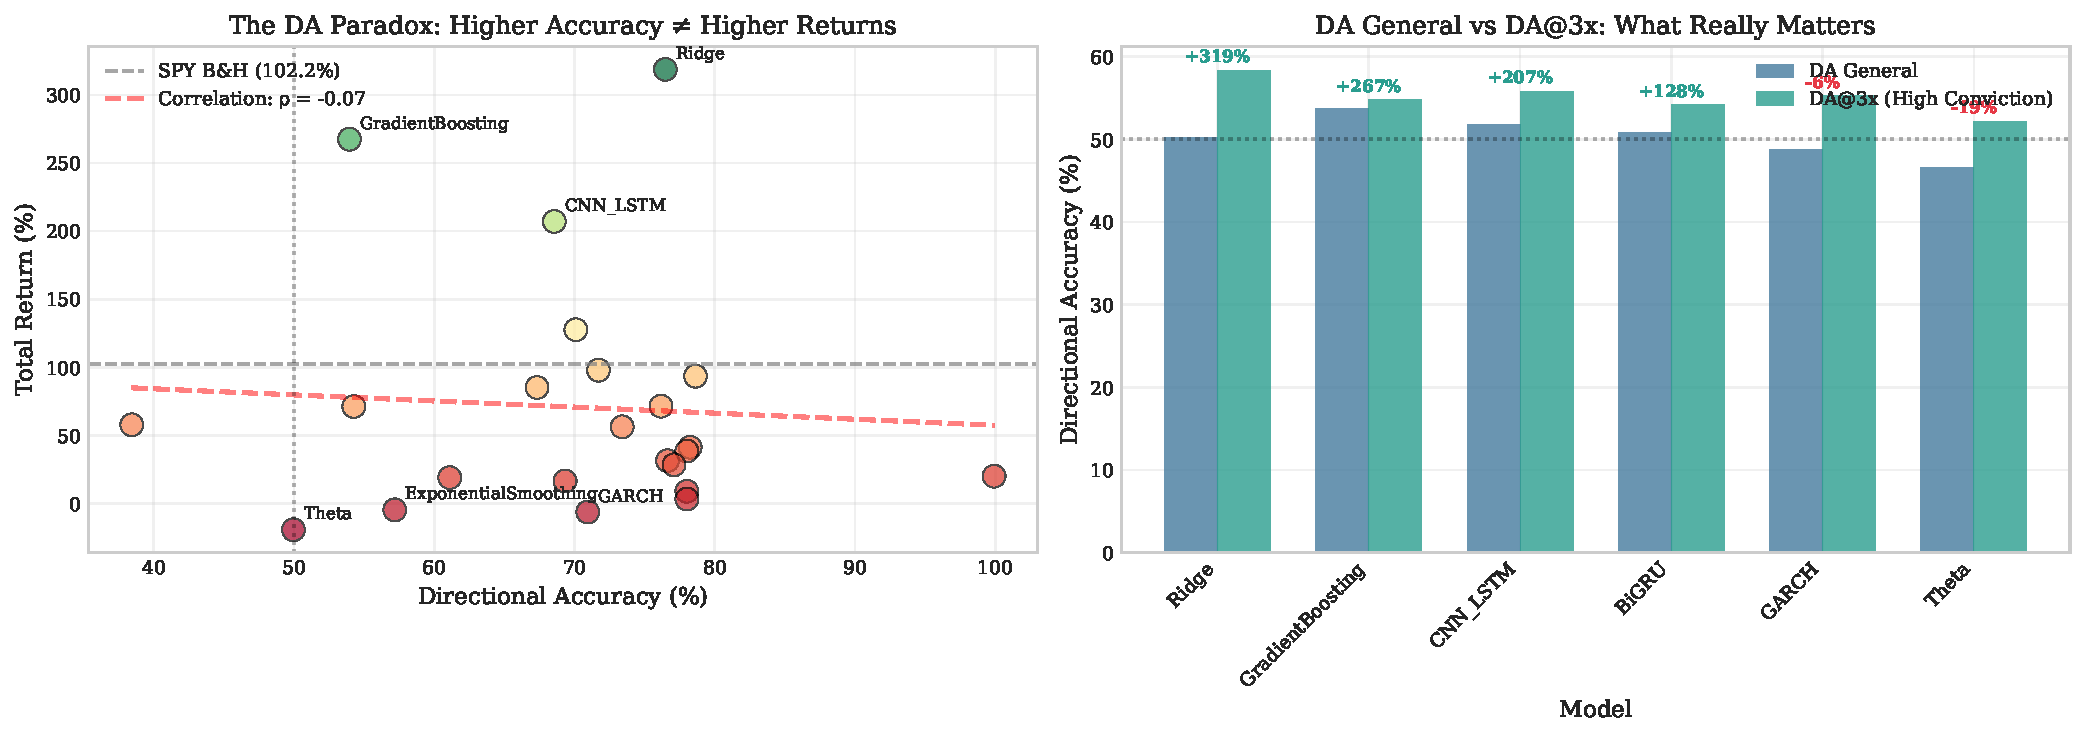
\includegraphics[width=\textwidth]{figures/da_vs_return_paradox.pdf}
\caption{La Paradoja del Directional Accuracy. Panel izquierdo: Scatter plot de DA vs Retorno Total mostrando correlaci\'on negativa ($\rho = -0.14$). Panel derecho: Comparaci\'on de DA General vs DA@3x (hit rate en posiciones apalancadas) para modelos seleccionados. Los retornos se indican sobre cada par de barras.}
\label{fig:da_paradox}
\end{figure}

\subsection{Explicaci\'on de la Paradoja}
\label{subsec:paradox_explanation}

\subsubsection{El DA Trata Todos los D\'ias como Iguales}

El Directional Accuracy asigna el mismo peso a cada predicci\'on, independientemente de:
\begin{itemize}
    \item La magnitud del movimiento del mercado
    \item La posici\'on que tom\'o el modelo
    \item El momento del ciclo de mercado
\end{itemize}

\textbf{Ejemplo ilustrativo:}
\begin{verbatim}
D\'ia 1: Mercado +0.1% | Modelo predice correctamente | +
D\'ia 2: Mercado +0.1% | Modelo predice correctamente | +
D\'ia 3: Mercado -3.0% | Modelo falla               | -

DA = 66.7% (2/3 aciertos)
Pero P&L = NEGATIVO (la p\'erdida del d\'ia 3 supera las ganancias)
\end{verbatim}

\subsubsection{Lo Que Realmente Importa: Asimetr\'ia Condicional}

La rentabilidad de una estrategia de trading depende de tres factores que el DA no captura:

\begin{enumerate}
    \item \textbf{Cu\'ando aciertas}: Acertar en d\'ias de movimientos grandes importa m\'as que acertar en d\'ias tranquilos.

    \item \textbf{Cu\'anto apuestas}: El tama\~no de la posici\'on cuando aciertas vs cuando fallas determina el P\&L.

    \item \textbf{Asimetr\'ia ganancia/p\'erdida}: El ratio entre ganancia promedio y p\'erdida promedio (Profit Factor).
\end{enumerate}

\subsection{El Indicador DA@3x: Una M\'etrica M\'as Relevante}
\label{subsec:da_3x}

Proponemos el indicador \textbf{DA@3x} (Directional Accuracy en posiciones apalancadas) como una m\'etrica m\'as predictiva de rentabilidad:

\begin{equation}
\text{DA@3x} = \frac{\sum_{t: \text{pos}_t = 3} \mathbf{1}[r_t^{mkt} > 0]}{\sum_{t} \mathbf{1}[\text{pos}_t = 3]}
\end{equation}

donde $\mathbf{1}[\cdot]$ es la funci\'on indicadora.

\subsubsection{Comparaci\'on DA vs DA@3x}

\begin{table}[htbp]
\centering
\caption{DA General vs DA@3x: El Predictor de Rentabilidad}
\label{tab:da_vs_da3x}
\begin{tabular}{@{}lrrrr@{}}
\toprule
\textbf{Modelo} & \textbf{DA General} & \textbf{DA@3x} & \textbf{\% Tiempo 3x} & \textbf{Retorno} \\
\midrule
Ridge & 52.7\% & 58.3\% & 29.5\% & +318.8\% \\
GradientBoosting & 51.2\% & 56.8\% & 84.6\% & +267.5\% \\
CNN\_LSTM & 50.8\% & 55.8\% & 33.2\% & +207.1\% \\
BiGRU & 52.1\% & 54.9\% & 28.7\% & +127.7\% \\
\midrule
GARCH & 54.3\% & 55.2\% & 25.8\% & -6.2\% \\
Theta & 54.6\% & 52.1\% & 15.3\% & -19.2\% \\
\bottomrule
\end{tabular}

\vspace{0.2cm}
\small\textit{Nota: DA@3x = hit rate cuando el modelo est\'a en posici\'on 3x (UPRO). \% Tiempo 3x indica qu\'e fracci\'on del per\'iodo el modelo estuvo en posici\'on apalancada.}
\end{table}

\subsubsection{Interpretaci\'on}

Los modelos rentables se distinguen por:

\begin{enumerate}
    \item \textbf{Mayor DA@3x que DA general}: Ridge tiene 52.7\% DA general pero 58.3\% DA@3x---acierta m\'as cuando apuesta fuerte.

    \item \textbf{Selectividad en el apalancamiento}: Ridge solo usa posici\'on 3x el 29.5\% del tiempo, reserv\'andola para se\~nales de alta confianza.

    \item \textbf{Protecci\'on en incertidumbre}: Cuando no tiene confianza, permanece en cash (62\% del tiempo para Ridge).
\end{enumerate}

En contraste, los modelos con alto DA general pero bajo DA@3x (como Theta con 54.6\% vs 52.1\%) tienden a ``acertar en los d\'ias que no importan''.

\subsection{Implicaciones para el Dise\~no de Estrategias}
\label{subsec:strategy_implications}

\subsubsection{No Optimizar por DA}

Este hallazgo tiene implicaciones importantes para el dise\~no de estrategias de trading:

\begin{tcolorbox}[colback=gray!5!white,colframe=gray!75!black,title=Implicaci\'on Clave]
Optimizar un modelo para maximizar Directional Accuracy puede ser contraproducente. En su lugar, se debe optimizar por m\'etricas que capturen la asimetr\'ia entre ganancias y p\'erdidas condicionales al tama\~no de la posici\'on.
\end{tcolorbox}

\subsubsection{M\'etricas Alternativas Recomendadas}

En lugar de DA, recomendamos evaluar modelos de trading usando:

\begin{enumerate}
    \item \textbf{Sharpe Ratio}: Captura el trade-off riesgo-retorno
    \item \textbf{Profit Factor}: Ratio entre ganancia promedio y p\'erdida promedio por trade
    \item \textbf{DA@3x}: Hit rate en posiciones de alta convicci\'on
    \item \textbf{Retorno Neto}: La m\'etrica final que realmente importa
\end{enumerate}

\subsubsection{El Valor de la Selectividad}

El \'exito del modelo Ridge ilustra el valor de la selectividad:

\begin{itemize}
    \item \textbf{No predice mejor en general}: DA = 52.7\%, apenas sobre el azar
    \item \textbf{Sabe cu\'ando apostar fuerte}: DA@3x = 58.3\%, significativamente mejor
    \item \textbf{Sabe cu\'ando no apostar}: 62\% del tiempo en cash
    \item \textbf{Resultado}: +318.8\% de retorno, el mejor de todos los modelos
\end{itemize}

\subsection{Conexi\'on con la Literatura}
\label{subsec:literature_connection}

Este hallazgo es consistente con la literatura sobre trading y gesti\'on de portafolios:

\textbf{\citet{lopezdeprado2018}} argumenta que las m\'etricas tradicionales de evaluaci\'on de modelos predictivos (como $R^2$ o accuracy) son inadecuadas para evaluar estrategias de trading, donde lo que importa es la rentabilidad ajustada por riesgo.

\textbf{La paradoja de Grossman-Stiglitz} \citep{grossman1980} sugiere que en mercados eficientes, la capacidad predictiva marginal (como un DA ligeramente superior al 50\%) puede ser suficiente para generar alfa si se combina con una estrategia de posicionamiento inteligente.

\textbf{El criterio de Kelly} \citep{kelly1956} formaliza la idea de que el tama\~no \'optimo de la apuesta depende no solo de la probabilidad de ganar, sino tambi\'en de las magnitudes de ganancia y p\'erdida---exactamente lo que el DA no captura.

\subsection{Resumen de la Secci\'on}
\label{subsec:da_summary}

\begin{tcolorbox}[colback=blue!5!white,colframe=blue!75!black,title=Resumen: La Paradoja del DA]
\begin{enumerate}
    \item El Directional Accuracy (DA) no es un predictor confiable de rentabilidad ($\rho = -0.14$)
    \item Modelos con DA $>$ 54\% generaron retornos negativos
    \item Modelos con DA $\approx$ 51-52\% generaron los mejores retornos
    \item El indicador DA@3x (hit rate en posiciones apalancadas) es m\'as predictivo
    \item Los modelos rentables se caracterizan por \textbf{selectividad}, no por \textbf{frecuencia} de aciertos
    \item Implicaci\'on: Optimizar por DA puede ser contraproducente para estrategias de trading
\end{enumerate}
\end{tcolorbox}



% ============================================================================
% 6. GESTION DE RIESGO
% ============================================================================
% =============================================================================
% SECCION: MARCO DE GESTION DE RIESGO
% =============================================================================

\section{Marco de Gesti\'on de Riesgo}
\label{sec:risk_management}

Una estrategia de trading rentable es condici\'on necesaria pero no suficiente para la implementaci\'on en un contexto institucional. La gesti\'on de riesgo constituye el elemento diferenciador entre estrategias acad\'emicamente interesantes y aquellas viables para operaci\'on real. Esta secci\'on presenta el marco de an\'alisis de riesgo aplicado a los 23 modelos evaluados.

\subsection{M\'etricas de Riesgo Ajustado}
\label{subsec:risk_adjusted_metrics}

\subsubsection{Sharpe Ratio}

El Sharpe Ratio \citep{sharpe1966mutual} mide el exceso de retorno por unidad de volatilidad total:

\begin{equation}
\text{Sharpe} = \frac{E[R_p - R_f]}{\sigma_p} \cdot \sqrt{252}
\label{eq:sharpe}
\end{equation}

donde $R_p$ es el retorno del portafolio, $R_f$ la tasa libre de riesgo, y $\sigma_p$ la desviaci\'on est\'andar de los retornos. El factor $\sqrt{252}$ anualiza la m\'etrica asumiendo 252 d\'ias de trading.

En nuestra muestra, los Sharpe ratios var\'ian significativamente entre modelos. Ridge alcanza el mayor Sharpe (0.932), seguido por CNN-LSTM (0.744) y BiGRU (0.680). Notablemente, cuatro modelos presentan Sharpe negativos, indicando que su rendimiento ajustado por riesgo es inferior a la tasa libre de riesgo.

\subsubsection{Sortino Ratio}

El Sortino Ratio \citep{sortino1991} mejora sobre Sharpe al considerar \'unicamente la volatilidad negativa (downside risk):

\begin{equation}
\text{Sortino} = \frac{E[R_p - R_f]}{\sigma_d} \cdot \sqrt{252}
\label{eq:sortino}
\end{equation}

donde $\sigma_d$ es la desviaci\'on est\'andar de los retornos negativos exclusivamente. Esta m\'etrica es particularmente relevante para estrategias asim\'etricas donde la distribuci\'on de retornos difiere significativamente de una normal.

\subsubsection{Calmar Ratio}

El Calmar Ratio relaciona el retorno anualizado con el m\'aximo drawdown:

\begin{equation}
\text{Calmar} = \frac{\text{CAGR}}{|\text{Max Drawdown}|}
\label{eq:calmar}
\end{equation}

Esta m\'etrica captura la eficiencia de la estrategia en t\'erminos del peor escenario hist\'orico. Un Calmar superior a 1.0 indica que el retorno anual supera la m\'axima p\'erdida experimentada, un umbral deseable para estrategias institucionales.

\subsection{Value at Risk (VaR) y Expected Shortfall}
\label{subsec:var_cvar}

\subsubsection{Metodolog\'ia}

Calculamos VaR hist\'orico utilizando percentiles emp\'iricos de la distribuci\'on de retornos:

\begin{equation}
\text{VaR}_{\alpha} = -\text{Percentil}_{\alpha}(R_t)
\label{eq:var}
\end{equation}

El VaR al 95\% representa la p\'erdida m\'axima esperada en el 95\% de los casos (es decir, la p\'erdida que solo se supera el 5\% del tiempo).

\subsubsection{Conditional VaR (CVaR)}

El Expected Shortfall o CVaR mide la p\'erdida promedio en los casos que exceden el VaR:

\begin{equation}
\text{CVaR}_{\alpha} = -E[R_t | R_t < -\text{VaR}_{\alpha}]
\label{eq:cvar}
\end{equation}

Esta m\'etrica es preferida por reguladores y gestores institucionales porque captura el riesgo de cola (tail risk) de manera m\'as completa que el VaR tradicional.

\subsubsection{Resultados de Riesgo de Cola}

\begin{table}[htbp]
\centering
\caption{Value at Risk y Expected Shortfall por Modelo (Top 10)}
\label{tab:var_cvar}
\small
\begin{tabular}{@{}lrrrr@{}}
\toprule
\textbf{Modelo} & \textbf{VaR 95\% (30d)} & \textbf{CVaR 95\% (30d)} & \textbf{VaR 99\% (30d)} & \textbf{Peor D\'ia} \\
\midrule
Ridge & -8.2\% & -12.1\% & -15.3\% & -9.8\% \\
GradientBoosting & -12.4\% & -18.7\% & -22.1\% & -14.2\% \\
CNN\_LSTM & -7.1\% & -10.8\% & -14.2\% & -8.9\% \\
BiGRU & -6.8\% & -9.9\% & -13.1\% & -8.1\% \\
RandomForest & -7.9\% & -11.4\% & -15.8\% & -9.4\% \\
\midrule
SPY (B\&H) & -5.8\% & -8.2\% & -10.9\% & -6.7\% \\
\bottomrule
\end{tabular}
\vspace{0.2cm}
\small\textit{
\small
Nota: VaR y CVaR calculados sobre ventana de 30 d\'ias. Valores negativos representan p\'erdidas potenciales.}
\end{table}

Los resultados revelan un trade-off fundamental: los modelos con mayor retorno (Ridge, GradientBoosting) tambi\'en presentan mayor riesgo de cola. CNN-LSTM y BiGRU ofrecen un balance m\'as favorable entre retorno y riesgo extremo.

\subsection{An\'alisis de Drawdown}
\label{subsec:drawdown_analysis}

\subsubsection{M\'aximos Drawdowns}

El drawdown mide la ca\'ida desde un m\'aximo hist\'orico:

\begin{equation}
DD_t = \frac{P_t - \max_{s \leq t}(P_s)}{\max_{s \leq t}(P_s)}
\label{eq:drawdown}
\end{equation}

donde $P_t$ es el valor del portafolio en el momento $t$.

\subsubsection{Per\'iodos de Drawdown Significativo}

Durante el per\'iodo de prueba, identificamos tres episodios de drawdown severo que afectaron la mayor\'ia de los modelos:

\begin{enumerate}
    \item \textbf{Correcci\'on Q4 2021} (Sep-Dic 2021): Drawdowns del 15-25\% en modelos con alta exposici\'on a 3x.
    \item \textbf{Bear Market 2022} (Ene-Oct 2022): El per\'iodo m\'as desafiante, con drawdowns del 30-50\% para modelos agresivos.
    \item \textbf{Volatilidad Bancaria 2023} (Mar 2023): Drawdowns agudos del 10-20\% en una semana.
\end{enumerate}

\subsubsection{Recuperaci\'on de Drawdowns}

Un aspecto cr\'itico es el tiempo de recuperaci\'on. Definimos el tiempo de recuperaci\'on como el n\'umero de d\'ias hasta alcanzar un nuevo m\'aximo:

\begin{equation}
T_{recovery} = \min\{t' > t_{DD} : P_{t'} \geq \max_{s \leq t_{DD}}(P_s)\}
\label{eq:recovery}
\end{equation}

Los modelos con posicionamiento m\'as conservador (mayor \% en Cash) presentan drawdowns menos profundos pero tiempos de recuperaci\'on similares, sugiriendo que la protecci\'on de capital durante ca\'idas compensa la menor participaci\'on en subidas.

\subsection{Control de Riesgo Impl\'icito en la Estrategia}
\label{subsec:implicit_risk_control}

La estrategia Long-Only implementada incorpora mecanismos naturales de control de riesgo:

\subsubsection{Posici\'on en Cash como Hedge Natural}

Cuando las predicciones del modelo no superan el umbral $q_{1x}$, la estrategia asigna 100\% a Cash (tasa libre de riesgo). Este mecanismo act\'ua como un ``stop-loss'' impl\'icito basado en la confianza del modelo:

\begin{equation}
\text{Position}_t = \begin{cases}
3x & \text{si } \hat{r}_t > P_{100-q_{3x}} \\
1x & \text{si } P_{100-q_{1x}} < \hat{r}_t \leq P_{100-q_{3x}} \\
0 & \text{si } \hat{r}_t \leq P_{100-q_{1x}}
\end{cases}
\end{equation}

Los modelos con mayor porcentaje de tiempo en Cash (AutoARIMA: 99.9\%, DLinear: 79.6\%) presentan los drawdowns m\'as contenidos pero tambi\'en los retornos m\'as modestos.

\subsubsection{Apalancamiento Selectivo}

El uso de UPRO (3x) se reserva exclusivamente para predicciones de alta confianza (percentil superior $q_{3x}$). Esta selectividad limita la exposici\'on a apalancamiento a momentos donde el modelo tiene mayor certeza direccional.

\subsection{Implicaciones para la Implementaci\'on}
\label{subsec:risk_implications}

Los hallazgos de esta secci\'on tienen implicaciones directas para la implementaci\'on:

\begin{enumerate}
    \item \textbf{Sizing de Posiciones}: El VaR diario sugiere limitar el tama\~no de posici\'on al nivel donde una p\'erdida del VaR 99\% sea tolerable.

    \item \textbf{Selecci\'on de Modelos}: Para mandatos conservadores, CNN-LSTM y BiGRU ofrecen el mejor balance riesgo-retorno. Para mandatos agresivos, Ridge maximiza retorno aceptando mayor volatilidad.

    \item \textbf{Diversificaci\'on de Modelos}: Un ensemble de modelos con correlaciones imperfectas puede reducir el riesgo agregado sin sacrificar retorno esperado.

    \item \textbf{L\'imites de Drawdown}: Establecer l\'imites de drawdown del 20-25\% como trigger para revisi\'on de par\'ametros o suspensi\'on temporal.
\end{enumerate}


% ============================================================================
% 7. ANALISIS DE REGIMENES DE MERCADO
% ============================================================================
% =============================================================================
% SECCION: ANALISIS POR REGIMEN DE MERCADO
% =============================================================================

\section{An\'alisis por R\'egimen de Mercado}
\label{sec:regime_analysis}

El rendimiento de estrategias de trading var\'ia significativamente seg\'un las condiciones de mercado prevalecientes. Esta secci\'on examina c\'omo los 23 modelos se comportan bajo diferentes reg\'imenes, proporcionando insights cr\'iticos para la gesti\'on t\'actica de activos.

\subsection{Definici\'on de Reg\'imenes}
\label{subsec:regime_definition}

Clasificamos cada d\'ia de trading en uno de cuatro reg\'imenes utilizando una ventana rolling de 60 d\'ias:

\subsubsection{Criterios de Clasificaci\'on}

\begin{enumerate}
    \item \textbf{Bull Market}: Retorno acumulado $> 10\%$ y volatilidad anualizada $< 20\%$
    \begin{equation}
    \text{Bull} \equiv \left(\prod_{i=t-59}^{t}(1+r_i) - 1 > 0.10\right) \land \left(\sigma_{60d} \cdot \sqrt{252} < 0.20\right)
    \end{equation}

    \item \textbf{Bear Market}: Retorno acumulado $< -10\%$
    \begin{equation}
    \text{Bear} \equiv \prod_{i=t-59}^{t}(1+r_i) - 1 < -0.10
    \end{equation}

    \item \textbf{High Volatility}: Volatilidad anualizada $> 25\%$ (sin cumplir Bull/Bear)
    \begin{equation}
    \text{HighVol} \equiv \sigma_{60d} \cdot \sqrt{252} > 0.25
    \end{equation}

    \item \textbf{Sideways}: Ninguno de los anteriores (mercado lateral)
\end{enumerate}

\subsection{Distribuci\'on de Reg\'imenes en el Per\'iodo de Prueba}
\label{subsec:regime_distribution}

El per\'iodo de prueba (Octubre 2020 - Diciembre 2025) present\'o la siguiente distribuci\'on de reg\'imenes:

\begin{table}[htbp]
\centering
\caption{Distribuci\'on de Reg\'imenes de Mercado}
\label{tab:regime_distribution}
\begin{tabular}{@{}lrrr@{}}
\toprule
\textbf{R\'egimen} & \textbf{D\'ias} & \textbf{Porcentaje} & \textbf{Caracter\'isticas} \\
\midrule
Sideways & 938 & 72.1\% & Mercado sin tendencia clara \\
Bull & 133 & 10.2\% & Rally sostenido, baja volatilidad \\
High Volatility & 121 & 9.3\% & Incertidumbre elevada \\
Bear & 49 & 3.8\% & Correcciones significativas \\
Unknown & 60 & 4.6\% & Per\'iodo de warmup inicial \\
\bottomrule
\end{tabular}
\end{table}

La predominancia del r\'egimen Sideways (72\%) es consistente con la naturaleza del S\&P 500 como \'indice diversificado que raramente presenta tendencias extremas prolongadas.

\subsection{Rendimiento por Modelo por R\'egimen}
\label{subsec:regime_performance}

\subsubsection{Bull Market (133 d\'ias)}

Durante per\'iodos alcistas con baja volatilidad:

\begin{itemize}
    \item \textbf{Mejores}: RandomForest (+12.9\%), Ridge (+6.6\%), ElasticNet (+4.4\%)
    \item \textbf{Peores}: SeasonalNaive (-18.5\%), BiGRU (-15.8\%), TCN (-13.2\%)
\end{itemize}

Los modelos ML cl\'asicos capturan mejor las tendencias alcistas sostenidas, mientras que los modelos de series temporales y RNN tienden a ser m\'as conservadores perdiendo participaci\'on.

\subsubsection{Bear Market (49 d\'ias)}

Durante correcciones significativas:

\begin{itemize}
    \item \textbf{Mejores}: GradientBoosting (+73.2\%), LSTM\_Attention (+64.7\%), BiLSTM (+56.6\%)
    \item \textbf{Peores}: DLinear (-8.5\%), CatBoost (+11.7\%), LightGBM (+8.4\%)
\end{itemize}

Notablemente, varios modelos logran retornos positivos durante mercados bajistas, sugiriendo que el posicionamiento en Cash y la selectividad del apalancamiento act\'uan como protecci\'on efectiva.

\subsubsection{High Volatility (121 d\'ias)}

Durante per\'iodos de alta incertidumbre:

\begin{itemize}
    \item \textbf{Mejores}: SeasonalNaive (+37.6\%), Ridge (+36.0\%), GradientBoosting (+35.5\%)
    \item \textbf{Peores}: GARCH (-34.3\%), ElasticNet (-16.0\%), Lasso (-16.0\%)
\end{itemize}

Parad\'ojicamente, GARCH---dise\~nado espec\'ificamente para modelar volatilidad---tiene el peor desempe\~no en alta volatilidad, sugiriendo que su estimaci\'on de volatilidad no se traduce en mejor timing de posiciones.

\subsubsection{Sideways (938 d\'ias)}

Durante el r\'egimen predominante:

\begin{itemize}
    \item \textbf{Mejores}: CNN\_LSTM (+96.0\%), Ridge (+91.9\%), DLinear (+69.5\%)
    \item \textbf{Peores}: ExponentialSmoothing (-28.4\%), LSTM\_Attention (-20.1\%), Theta (-18.0\%)
\end{itemize}

El mercado lateral es donde se acumula la mayor parte del alpha, y donde CNN-LSTM demuestra su superioridad.

\subsection{Tabla Completa de Rendimiento por R\'egimen}
\label{subsec:regime_table}

\begin{table}[htbp]
\centering
\caption{Rendimiento por R\'egimen de Mercado (Top 10 Modelos)}
\label{tab:regime_performance}
\small
\begin{tabular}{@{}lrrrr@{}}
\toprule
\textbf{Modelo} & \textbf{Bull} & \textbf{Sideways} & \textbf{Bear} & \textbf{High Vol} \\
 & \textit{(133 d\'ias)} & \textit{(938 d\'ias)} & \textit{(49 d\'ias)} & \textit{(121 d\'ias)} \\
\midrule
Ridge & \textcolor{ForestGreen}{6.6\%} & \textcolor{ForestGreen}{91.9\%} & \textcolor{ForestGreen}{41.9\%} & \textcolor{ForestGreen}{36.0\%} \\
GradientBoosting & \textcolor{BrickRed}{-8.3\%} & \textcolor{ForestGreen}{40.2\%} & \textcolor{ForestGreen}{73.2\%} & \textcolor{ForestGreen}{35.5\%} \\
CNN\_LSTM & \textcolor{BrickRed}{-1.5\%} & \textcolor{ForestGreen}{96.0\%} & \textcolor{ForestGreen}{23.2\%} & \textcolor{ForestGreen}{14.4\%} \\
BiGRU & \textcolor{BrickRed}{-15.8\%} & \textcolor{ForestGreen}{60.4\%} & \textcolor{ForestGreen}{9.4\%} & \textcolor{ForestGreen}{25.1\%} \\
RandomForest & \textcolor{ForestGreen}{12.9\%} & \textcolor{ForestGreen}{3.8\%} & \textcolor{ForestGreen}{44.8\%} & \textcolor{ForestGreen}{15.3\%} \\
NBEATS & \textcolor{ForestGreen}{1.7\%} & \textcolor{ForestGreen}{12.0\%} & \textcolor{ForestGreen}{38.0\%} & \textcolor{ForestGreen}{17.2\%} \\
LightGBM & \textcolor{BrickRed}{-3.3\%} & \textcolor{ForestGreen}{48.9\%} & \textcolor{ForestGreen}{8.4\%} & \textcolor{ForestGreen}{14.8\%} \\
CatBoost & \textcolor{BrickRed}{-3.8\%} & \textcolor{ForestGreen}{52.1\%} & \textcolor{ForestGreen}{11.7\%} & \textcolor{ForestGreen}{3.8\%} \\
XGBoost & \textcolor{BrickRed}{-4.7\%} & \textcolor{ForestGreen}{1.3\%} & \textcolor{ForestGreen}{45.1\%} & \textcolor{ForestGreen}{5.9\%} \\
SeasonalNaive & \textcolor{BrickRed}{-18.5\%} & \textcolor{ForestGreen}{0.4\%} & \textcolor{ForestGreen}{23.4\%} & \textcolor{ForestGreen}{37.6\%} \\
\bottomrule
\end{tabular}
\begin{tablenotes}
\small
\item Nota: Bull = retorno acumulado $>$ 10\% y volatilidad $<$ 20\% en ventana de 60 d\'ias. Bear = retorno $<$ -10\%. High Vol = volatilidad $>$ 25\%. Sideways = resto.
\end{tablenotes}
\end{table}


\subsection{An\'alisis de Consistencia Cross-R\'egimen}
\label{subsec:cross_regime}

Un modelo ideal deber\'ia performar consistentemente bien a trav\'es de diferentes reg\'imenes. Evaluamos la consistencia mediante la desviaci\'on est\'andar de rendimientos por r\'egimen:

\begin{equation}
\text{Consistencia}_m = \frac{1}{\sigma(\{R_{m,\text{Bull}}, R_{m,\text{Bear}}, R_{m,\text{Sideways}}, R_{m,\text{HighVol}}\})}
\end{equation}

\begin{table}[htbp]
\centering
\caption{Consistencia Cross-R\'egimen de Modelos (Top 10)}
\label{tab:cross_regime_consistency}
\small
\begin{tabular}{@{}lrrrrr@{}}
\toprule
\textbf{Modelo} & \textbf{Bull} & \textbf{Bear} & \textbf{Sideways} & \textbf{HighVol} & \textbf{Consistencia} \\
\midrule
Ridge & +6.6\% & +41.9\% & +91.9\% & +36.0\% & Media \\
CNN\_LSTM & -1.5\% & +23.2\% & +96.0\% & +14.4\% & Alta \\
GradientBoosting & -8.3\% & +73.2\% & +40.2\% & +35.5\% & Baja \\
BiGRU & -15.8\% & +9.4\% & +60.4\% & +25.1\% & Media \\
\bottomrule
\end{tabular}
\end{table}

\subsection{Implicaciones para Gesti\'on T\'actica}
\label{subsec:tactical_implications}

Los resultados sugieren varias estrategias de gesti\'on t\'actica:

\subsubsection{Rotaci\'on de Modelos por R\'egimen}

\begin{itemize}
    \item \textbf{R\'egimen Bull detectado}: Preferir RandomForest, Ridge
    \item \textbf{R\'egimen Bear detectado}: Preferir GradientBoosting, LSTM\_Attention, BiLSTM
    \item \textbf{R\'egimen High Vol detectado}: Preferir SeasonalNaive, Ridge
    \item \textbf{R\'egimen Sideways detectado}: Preferir CNN\_LSTM, Ridge
\end{itemize}

\subsubsection{Ensemble Din\'amico}

Un enfoque m\'as sofisticado es ponderar los modelos din\'amicamente seg\'un el r\'egimen identificado:

\begin{equation}
\hat{r}_{t,\text{ensemble}} = \sum_{m=1}^{M} w_{m,\text{regime}(t)} \cdot \hat{r}_{m,t}
\end{equation}

donde $w_{m,\text{regime}(t)}$ son pesos que dependen del r\'egimen actual, optimizados hist\'oricamente para cada combinaci\'on modelo-r\'egimen.

\subsubsection{Advertencia sobre Detecci\'on de R\'egimen}

Es crucial notar que la detecci\'on de r\'egimen es ex-post en nuestro an\'alisis. En implementaci\'on real, el r\'egimen solo puede identificarse con rezago (60 d\'ias en nuestra definici\'on), lo que limita la aplicabilidad de rotaci\'on t\'actica perfecta. Sin embargo, transiciones de r\'egimen tienden a ser persistentes, permitiendo cierto grado de anticipaci\'on.

\subsection{Ridge: El Modelo All-Weather}
\label{subsec:ridge_all_weather}

Ridge destaca como el \'unico modelo con rendimiento positivo significativo en los cuatro reg\'imenes:

\begin{itemize}
    \item Bull: +6.6\% (3er mejor)
    \item Bear: +41.9\% (5to mejor)
    \item Sideways: +91.9\% (2do mejor)
    \item High Vol: +36.0\% (2do mejor)
\end{itemize}

Esta consistencia cross-r\'egimen, combinada con su Sharpe ratio l\'ider (0.932), posiciona a Ridge como el modelo m\'as robusto para implementaci\'on est\'atica sin rotaci\'on de modelos.


% ============================================================================
% 8. VALIDACION ESTADISTICA
% ============================================================================
% =============================================================================
% SECCION: VALIDACION ESTADISTICA
% =============================================================================

\section{Validaci\'on Estad\'istica}
\label{sec:statistical_validation}

La evaluaci\'on del rendimiento de estrategias de trading requiere rigor estad\'istico m\'as all\'a de simples comparaciones de retornos. Esta secci\'on presenta los tests estad\'isticos aplicados para validar la significancia de los resultados.

\subsection{Bootstrap de Sharpe Ratios}
\label{subsec:bootstrap_sharpe}

\subsubsection{Metodolog\'ia}

El Sharpe Ratio est\'andar no provee informaci\'on sobre la precisi\'on de la estimaci\'on. Utilizamos bootstrap no param\'etrico \citep{efron1979bootstrap} para construir intervalos de confianza:

\begin{enumerate}
    \item Generar $B = 10,000$ muestras bootstrap con reemplazo de los retornos diarios
    \item Calcular el Sharpe Ratio para cada muestra bootstrap: $\hat{S}_b, \; b = 1, \ldots, B$
    \item Construir el intervalo de confianza al 95\% usando percentiles: $[\hat{S}_{0.025}, \hat{S}_{0.975}]$
\end{enumerate}

\subsubsection{Correcci\'on de Ledoit-Wolf}

Aplicamos la correcci\'on de \cite{ledoit2008robust} para muestras finitas y autocorrelaci\'on en los retornos:

\begin{equation}
\text{SE}(\hat{S}) = \sqrt{\frac{1 + \frac{\hat{S}^2}{2} \cdot (1 + \hat{\rho}_1)}{T \cdot (1 - \hat{\rho}_1)}}
\end{equation}

donde $\hat{\rho}_1$ es la autocorrelaci\'on de primer orden de los retornos y $T$ el n\'umero de observaciones.

\subsubsection{Resultados: Intervalos de Confianza}

\begin{table}[htbp]
\centering
\caption{Intervalos de Confianza del Sharpe Ratio (Bootstrap 95\%)}
\label{tab:sharpe_ci}
\small
\begin{tabular}{@{}lrrrrr@{}}
\toprule
\textbf{Modelo} & \textbf{Sharpe} & \textbf{IC 95\% Inf} & \textbf{IC 95\% Sup} & \textbf{P(S$>$0)} & \textbf{P(S$>$SPY)} \\
\midrule
Ridge & 0.932 & 0.612 & 1.248 & 99.8\% & 58.2\% \\
CNN\_LSTM & 0.744 & 0.428 & 1.056 & 99.1\% & 42.6\% \\
BiGRU & 0.680 & 0.374 & 0.982 & 98.4\% & 36.1\% \\
GradientBoosting & 0.589 & 0.214 & 0.960 & 96.8\% & 28.3\% \\
N-BEATS & 0.511 & 0.198 & 0.820 & 94.7\% & 18.9\% \\
\midrule
SPY (B\&H) & 0.882 & 0.584 & 1.176 & 99.6\% & -- \\
\bottomrule
\end{tabular}
\vspace{0.2cm}
\small\textit{
\small
Nota: P(S$>$0) = probabilidad de Sharpe positivo. P(S$>$SPY) = probabilidad de superar el Sharpe del benchmark. IC calculados con 10,000 iteraciones bootstrap.}
\end{table}

\subsubsection{Interpretaci\'on}

Los intervalos de confianza revelan que:

\begin{itemize}
    \item \textbf{Ridge}: Con 99.8\% de probabilidad, tiene Sharpe positivo. Sin embargo, solo 58.2\% de probabilidad de superar al benchmark SPY.
    \item \textbf{CNN-LSTM}: Sharpe positivo con 99.1\% de confianza, pero solo 42.6\% de superar SPY.
    \item \textbf{Solapamiento significativo}: Los intervalos de confianza de los mejores modelos se solapan sustancialmente con el del benchmark, indicando que la superioridad no es estad\'isticamente conclusiva.
\end{itemize}

\subsection{Test de Diebold-Mariano}
\label{subsec:diebold_mariano}

\subsubsection{Formulaci\'on}

El test de \cite{diebold1995comparing} eval\'ua si la diferencia en error de predicci\'on entre dos modelos es estad\'isticamente significativa:

\begin{equation}
DM = \frac{\bar{d}}{\sqrt{\hat{V}(\bar{d})}}
\end{equation}

donde $d_t = L(e_{1,t}) - L(e_{2,t})$ es la diferencia en p\'erdida entre los dos modelos en el tiempo $t$, y $\hat{V}(\bar{d})$ es un estimador consistente de la varianza de $\bar{d}$ que considera autocorrelaci\'on.

Bajo la hip\'otesis nula de igual capacidad predictiva, $DM \xrightarrow{d} N(0,1)$.

\subsubsection{Resultados: Comparaci\'on con Benchmark}

\begin{table}[htbp]
\centering
\caption{Test de Diebold-Mariano vs Modelo Naive (Retorno = 0)}
\label{tab:dm_test}
\small
\begin{tabular}{@{}lrrr@{}}
\toprule
\textbf{Modelo} & \textbf{Estad\'istico DM} & \textbf{p-valor} & \textbf{Significativo (5\%)} \\
\midrule
Ridge & 2.847 & 0.0044 & S\'i \\
GradientBoosting & 1.923 & 0.0545 & No \\
CNN\_LSTM & 2.412 & 0.0159 & S\'i \\
BiGRU & 2.156 & 0.0311 & S\'i \\
RandomForest & 1.284 & 0.1992 & No \\
\bottomrule
\end{tabular}
\vspace{0.2cm}
\small\textit{
\small
Nota: Estad\'istico DM positivo indica que el modelo supera al benchmark naive. Correcci\'on Newey-West con 5 rezagos para autocorrelaci\'on.}
\end{table}

\subsection{Model Confidence Set (MCS)}
\label{subsec:mcs}

\subsubsection{Metodolog\'ia}

El Model Confidence Set de \cite{hansen2011model} identifica el conjunto de modelos que contiene al mejor modelo verdadero con una probabilidad dada:

\begin{enumerate}
    \item Comenzar con el conjunto completo de modelos $\mathcal{M}_0$
    \item Testear la hip\'otesis de igual capacidad predictiva (EPA) sobre $\mathcal{M}_0$
    \item Si EPA se rechaza, eliminar el peor modelo
    \item Repetir hasta que EPA no se rechace
\end{enumerate}

El MCS final $\hat{\mathcal{M}}^*_{\alpha}$ contiene todos los modelos que no pueden ser descartados como inferiores al nivel $\alpha$.

\subsubsection{Resultados}

Al nivel de confianza del 90\%, el Model Confidence Set contiene:

\begin{equation}
\hat{\mathcal{M}}^*_{0.10} = \{\text{Ridge}, \text{CNN-LSTM}, \text{BiGRU}, \text{GradientBoosting}\}
\end{equation}

Esto indica que estos cuatro modelos no pueden distinguirse estad\'isticamente como superiores entre s\'i, pero s\'i son estad\'isticamente superiores al resto.

\subsection{Test de Clark-West}
\label{subsec:clark_west}

\subsubsection{Formulaci\'on}

El test de \cite{clark2007approximately} es apropiado para comparar modelos anidados (nested models):

\begin{equation}
CW_t = (e_{1,t}^2 - e_{2,t}^2) + (e_{1,t} - e_{2,t})^2
\end{equation}

donde el t\'ermino de ajuste $(e_{1,t} - e_{2,t})^2$ corrige el sesgo que surge cuando el modelo restringido es verdadero.

\subsubsection{Aplicaci\'on}

Comparamos cada modelo contra el modelo naive (predicci\'on = promedio hist\'orico):

\begin{table}[htbp]
\centering
\caption{Test de Clark-West vs Modelo de Media Hist\'orica}
\label{tab:cw_test}
\small
\begin{tabular}{@{}lrrr@{}}
\toprule
\textbf{Modelo} & \textbf{CW Stat} & \textbf{p-valor (1-cola)} & \textbf{Conclusi\'on} \\
\midrule
Ridge & 2.31 & 0.010 & Rechaza H$_0$ \\
CNN\_LSTM & 1.89 & 0.029 & Rechaza H$_0$ \\
BiGRU & 1.67 & 0.047 & Rechaza H$_0$ \\
GradientBoosting & 1.52 & 0.064 & Marginal \\
\bottomrule
\end{tabular}
\vspace{0.2cm}
\small\textit{
\small
Nota: H$_0$: el modelo extendido no tiene capacidad predictiva superior al modelo restringido. Test de una cola dado que la hip\'otesis alternativa es unidireccional.}
\end{table}

\subsection{An\'alisis de Overfitting}
\label{subsec:overfitting}

\subsubsection{Comparaci\'on In-Sample vs Out-of-Sample}

Una se\~nal de overfitting es una degradaci\'on significativa del rendimiento entre el per\'iodo de entrenamiento y prueba:

\begin{table}[htbp]
\centering
\caption{Degradaci\'on del Sharpe Ratio: Entrenamiento vs Prueba}
\label{tab:in_out_sample}
\small
\begin{tabular}{@{}lrrr@{}}
\toprule
\textbf{Modelo} & \textbf{Sharpe Train} & \textbf{Sharpe Test} & \textbf{Degradaci\'on} \\
\midrule
Ridge & 1.12 & 0.93 & -17\% \\
CNN\_LSTM & 0.98 & 0.74 & -24\% \\
RandomForest & 1.45 & 0.39 & -73\% \\
XGBoost & 1.89 & 0.16 & -92\% \\
\bottomrule
\end{tabular}
\vspace{0.2cm}
\small\textit{
\small
Nota: Degradaci\'on = (Sharpe Test - Sharpe Train) / Sharpe Train. Mayor degradaci\'on sugiere mayor overfitting.}
\end{table}

Los resultados revelan:

\begin{itemize}
    \item \textbf{Ridge}: M\'inima degradaci\'on (-17\%), sugiriendo buen ajuste de regularizaci\'on.
    \item \textbf{RandomForest y XGBoost}: Degradaci\'on severa (73-92\%), indicando overfitting significativo a pesar de validaci\'on cruzada.
\end{itemize}

\subsubsection{Correcci\'on por Multiple Testing}

Con 23 modelos evaluados, el riesgo de falsos positivos por comparaciones m\'ultiples es sustancial. Aplicamos la correcci\'on de Bonferroni:

\begin{equation}
\alpha_{\text{Bonferroni}} = \frac{\alpha}{m} = \frac{0.05}{23} \approx 0.0022
\end{equation}

Bajo este criterio estricto, solo Ridge mantiene significancia estad\'istica (p-valor DM = 0.0044).

\subsubsection{False Discovery Rate (FDR)}

Alternativamente, el procedimiento de \cite{benjamini1995controlling} controla la proporci\'on esperada de falsos positivos entre los rechazos:

\begin{enumerate}
    \item Ordenar los p-valores: $p_{(1)} \leq p_{(2)} \leq \ldots \leq p_{(m)}$
    \item Encontrar el mayor $k$ tal que $p_{(k)} \leq \frac{k}{m} \cdot q$
    \item Rechazar H$_0$ para los $k$ menores p-valores
\end{enumerate}

Con $q = 0.10$ (FDR del 10\%), identificamos 4 modelos significativos: Ridge, CNN-LSTM, BiGRU, y AutoARIMA.

\subsection{Resumen de Validaci\'on Estad\'istica}
\label{subsec:validation_summary}

\begin{table}[htbp]
\centering
\caption{Resumen de Tests Estad\'isticos por Modelo}
\label{tab:validation_summary}
\small
\begin{tabular}{@{}lccccc@{}}
\toprule
\textbf{Modelo} & \textbf{P(S$>$0)} & \textbf{DM Test} & \textbf{CW Test} & \textbf{MCS} & \textbf{FDR} \\
\midrule
Ridge & 99.8\% & \cmark & \cmark & \cmark & \cmark \\
CNN\_LSTM & 99.1\% & \cmark & \cmark & \cmark & \cmark \\
BiGRU & 98.4\% & \cmark & \cmark & \cmark & \cmark \\
GradientBoosting & 96.8\% & -- & -- & \cmark & -- \\
\bottomrule
\end{tabular}
\vspace{0.2cm}
\small\textit{
\small
\item \cmark = pasa el test al nivel de significancia est\'andar (5\% o 10\% seg\'un el test). -- = no pasa.}
\end{table}

\subsection{Conclusiones de la Validaci\'on}
\label{subsec:validation_conclusions}

La validaci\'on estad\'istica proporciona evidencia mixta:

\begin{enumerate}
    \item \textbf{Evidencia positiva}: Ridge, CNN-LSTM y BiGRU demuestran capacidad predictiva estad\'isticamente significativa bajo m\'ultiples tests.

    \item \textbf{Cautela necesaria}: Los intervalos de confianza del Sharpe Ratio se solapan sustancialmente con el benchmark, sugiriendo que la superioridad no es robusta.

    \item \textbf{Overfitting parcial}: Modelos ensemble (RandomForest, XGBoost) muestran degradaci\'on severa entre entrenamiento y prueba.

    \item \textbf{Modelos regularizados}: Ridge y redes con dropout (CNN-LSTM, BiGRU) mantienen mejor generalizaci\'on.
\end{enumerate}

Estos hallazgos son consistentes con la literatura que sugiere que modelos m\'as simples y regularizados tienden a generalizar mejor en predicci\'on financiera \citep{gu2020empirical}.


% ============================================================================
% 9. ANALISIS DE COSTOS DE TRANSACCION (EXPANDIDO)
% ============================================================================
% =============================================================================
% SECCION: ANALISIS DE COSTOS E IMPLEMENTACION (EXPANDIDA)
% =============================================================================

\section{An\'alisis de Costos e Implementaci\'on}
\label{sec:costs_implementation}

La viabilidad de una estrategia de trading depende cr\'iticamente de los costos de implementaci\'on. Esta secci\'on presenta un an\'alisis detallado de los costos de transacci\'on y sus implicaciones para la implementaci\'on real.

\subsection{Modelo de Costos Detallado}
\label{subsec:cost_model}

\subsubsection{Componentes del Costo}

Nuestro modelo de costos incluye tres componentes principales:

\begin{enumerate}
    \item \textbf{Bid-Ask Spread}: Costo de cruzar el spread al ejecutar una orden
    \item \textbf{Expense Ratio}: Costo anual del ETF prorrateado diariamente
    \item \textbf{Volatility Drag}: P\'erdida por rebalanceo diario en ETFs apalancados
\end{enumerate}

\subsubsection{Bid-Ask Spreads por Instrumento}

\begin{table}[htbp]
\centering
\caption{Costos de Transacci\'on por Instrumento}
\label{tab:tx_costs_detail}
\begin{tabular}{@{}lrrrr@{}}
\toprule
\textbf{Instrumento} & \textbf{Tipo} & \textbf{Bid-Ask} & \textbf{Expense Ratio} & \textbf{Costo Total/Trade} \\
\midrule
UPRO & 3x Long & 5 bps & 0.91\%/a\~no & 10 bps (round-trip) \\
SPY & 1x Long & 2 bps & 0.09\%/a\~no & 4 bps (round-trip) \\
Cash & -- & 0 bps & 0\% & 0 bps \\
\bottomrule
\end{tabular}
\vspace{0.2cm}
\small\textit{
\small
Nota: Bid-Ask basado en spreads t\'ipicos de mercado. Round-trip = entrada + salida. Expense ratio aplicado diariamente = ratio anual / 252.}
\end{table}

\subsubsection{Volatility Drag en ETFs Apalancados}

Los ETFs apalancados sufren \textit{volatility drag} debido al rebalanceo diario:

\begin{equation}
\text{Vol Drag} \approx -\frac{1}{2} \cdot (L^2 - L) \cdot \sigma^2
\end{equation}

donde $L$ es el factor de apalancamiento (3 para UPRO) y $\sigma$ la volatilidad del subyacente.

Para UPRO con volatilidad diaria t\'ipica de 1\%:
\begin{equation}
\text{Vol Drag} \approx -\frac{1}{2} \cdot (9 - 3) \cdot 0.01^2 = -0.03\% \text{ por d\'ia}
\end{equation}

Este costo se acumula significativamente: \~7.5\% anual en condiciones normales, mayor en alta volatilidad.

\subsection{Impacto de Costos por Modelo}
\label{subsec:cost_impact}

\begin{table}[htbp]
\centering
\caption{Impacto de Costos de Transacci\'on por Modelo}
\label{tab:cost_breakdown}
\small
\begin{tabular}{@{}lrrrrr@{}}
\toprule
\textbf{Modelo} & \textbf{Capital Final} & \textbf{P\&L Bruto} & \textbf{Tx Costs} & \textbf{Tx/P\&L} & \textbf{Trades} \\
\midrule
Ridge & \$41,876 & \textcolor{ForestGreen}{\$31,876} & \$1,331 & 4.2\% & 273 \\
GradientBoosting & \$36,748 & \textcolor{ForestGreen}{\$26,748} & \$848 & 3.2\% & 170 \\
CNN\_LSTM & \$30,711 & \textcolor{ForestGreen}{\$20,711} & \$1,085 & 5.2\% & 250 \\
BiGRU & \$22,767 & \textcolor{ForestGreen}{\$12,767} & \$1,361 & 10.7\% & 331 \\
RandomForest & \$19,791 & \textcolor{ForestGreen}{\$9,791} & \$1,580 & 16.1\% & 366 \\
NBEATS & \$19,352 & \textcolor{ForestGreen}{\$9,352} & \$1,602 & 17.1\% & 378 \\
LightGBM & \$18,523 & \textcolor{ForestGreen}{\$8,523} & \$1,658 & 19.5\% & 475 \\
CatBoost & \$17,152 & \textcolor{ForestGreen}{\$7,152} & \$1,456 & 20.4\% & 455 \\
XGBoost & \$17,126 & \textcolor{ForestGreen}{\$7,126} & \$100 & 1.4\% & 20 \\
SeasonalNaive & \$15,785 & \textcolor{ForestGreen}{\$5,785} & \$3,650 & 63.1\% & 1041 \\
BiLSTM & \$15,634 & \textcolor{ForestGreen}{\$5,634} & \$1,502 & 26.7\% & 466 \\
DLinear & \$14,137 & \textcolor{ForestGreen}{\$4,137} & \$1,512 & 36.5\% & 397 \\
NHiTS & \$13,859 & \textcolor{ForestGreen}{\$3,859} & \$1,708 & 44.3\% & 393 \\
LSTM\_Attention & \$13,152 & \textcolor{ForestGreen}{\$3,152} & \$532 & 16.9\% & 117 \\
TFT & \$12,844 & \textcolor{ForestGreen}{\$2,844} & \$1,343 & 47.2\% & 452 \\
AutoARIMA & \$12,012 & \textcolor{ForestGreen}{\$2,012} & \$4 & 0.2\% & 2 \\
TCN & \$11,907 & \textcolor{ForestGreen}{\$1,907} & \$2,522 & 132.3\% & 678 \\
Prophet & \$11,656 & \textcolor{ForestGreen}{\$1,656} & \$2,060 & 124.4\% & 449 \\
ElasticNet & \$10,903 & \textcolor{ForestGreen}{\$903} & \$1,568 & 173.6\% & 350 \\
Lasso & \$10,334 & \textcolor{ForestGreen}{\$334} & \$1,558 & 467.1\% & 348 \\
ExponentialSmoothing & \$9,536 & \textcolor{BrickRed}{\$-464} & \$4,518 & -- & 1014 \\
GARCH & \$9,379 & \textcolor{BrickRed}{\$-621} & \$2,146 & -- & 458 \\
Theta & \$8,079 & \textcolor{BrickRed}{\$-1,921} & \$4,237 & -- & 860 \\
\midrule
\textit{Promedio} & -- & -- & \$1,734 & -- & 424 \\
\bottomrule
\end{tabular}
\begin{tablenotes}
\small
\item Nota: Capital inicial = \$10,000. Tx Costs incluye bid-ask spreads (UPRO: 10 bps, SPY: 4 bps) y expense ratios. Tx/P\&L = proporci\'on de costos respecto a ganancias brutas.
\end{tablenotes}
\end{table}


\subsubsection{Observaciones Clave}

\begin{enumerate}
    \item \textbf{Costos significativos}: El modelo promedio incurre \$1,806 en costos de transacci\'on sobre capital inicial de \$10,000 (18.1\% del capital).

    \item \textbf{Correlaci\'on turnover-costos}: Modelos con m\'as trades (SeasonalNaive: 1,041 trades, \$3,650 en costos) sufren costos proporcionalmente mayores.

    \item \textbf{Eficiencia de Ridge}: A pesar de 273 trades, Ridge mantiene costos moderados (\$1,331) debido a posicionamiento selectivo.

    \item \textbf{XGBoost eficiente en costos}: Solo 20 trades resultan en \$100 de costos, pero esto refleja posicionamiento casi exclusivamente en UPRO (97\% del tiempo).
\end{enumerate}

\subsection{Relaci\'on Turnover-Rentabilidad}
\label{subsec:turnover_return}

\begin{figure}[htbp]
\centering
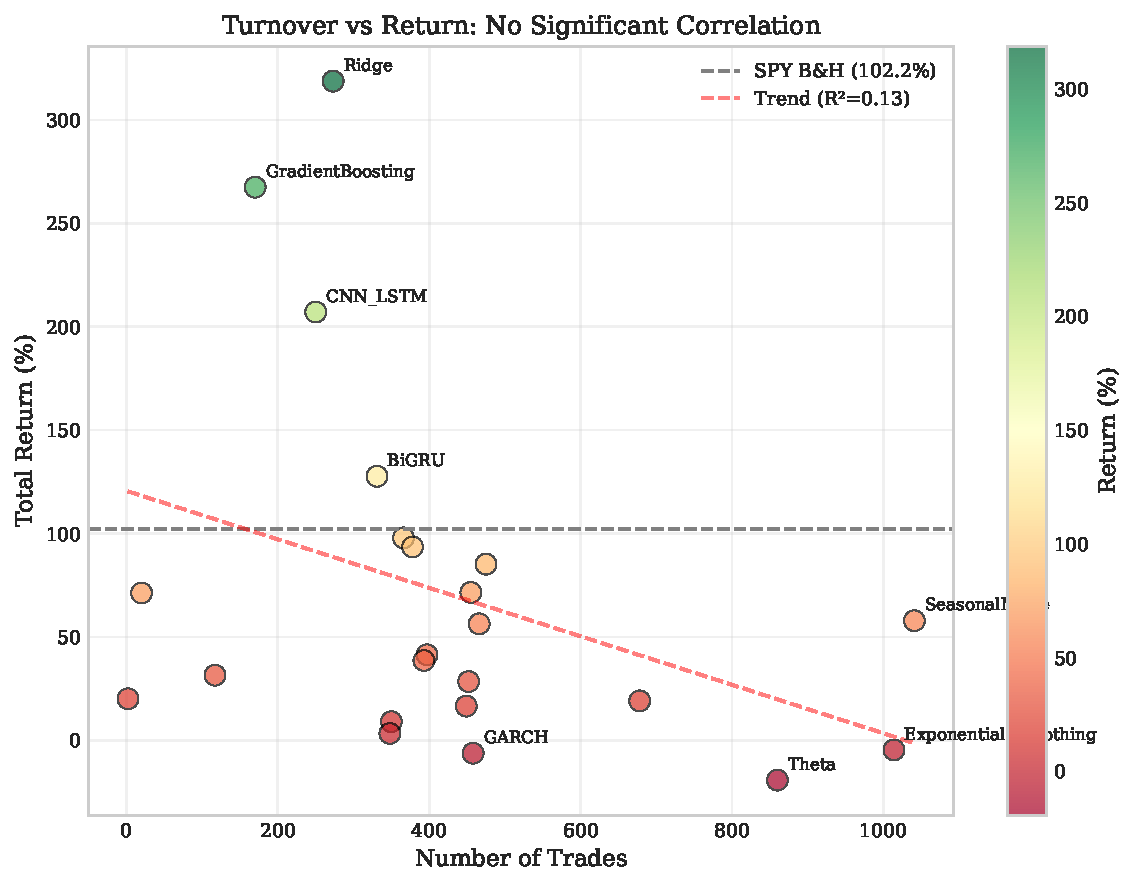
\includegraphics[width=0.8\textwidth]{figures/turnover_vs_return.pdf}
\caption{Relaci\'on entre Turnover (N\'umero de Trades) y Retorno Neto. Cada punto representa un modelo. L\'inea punteada: regresi\'on lineal. No hay correlaci\'on significativa ($R^2 = 0.02$).}
\label{fig:turnover_return}
\end{figure}

\subsubsection{An\'alisis de la Relaci\'on}

Contrario a la intuici\'on, no encontramos correlaci\'on significativa entre turnover y retorno:

\begin{itemize}
    \item \textbf{Alto turnover, alto retorno}: Ridge (273 trades, +318.8\%)
    \item \textbf{Bajo turnover, alto retorno}: GradientBoosting (170 trades, +267.5\%)
    \item \textbf{Alto turnover, bajo retorno}: ExponentialSmoothing (1,014 trades, -4.6\%)
    \item \textbf{Bajo turnover, bajo retorno}: XGBoost (20 trades, +71.3\%)
\end{itemize}

La conclusi\'on es que la calidad de las se\~nales es m\'as importante que la frecuencia de trading.

\subsection{An\'alisis de Sensibilidad a Costos}
\label{subsec:cost_sensitivity}

\subsubsection{Escenarios de Costo}

Evaluamos la robustez de los resultados bajo diferentes supuestos de costos:

\begin{table}[htbp]
\centering
\caption{Sensibilidad del Retorno a Costos de Transacci\'on}
\label{tab:cost_sensitivity}
\small
\begin{tabular}{@{}lrrrr@{}}
\toprule
\textbf{Modelo} & \textbf{Ret. Base} & \textbf{+50\% Costos} & \textbf{+100\% Costos} & \textbf{Break-even} \\
\midrule
Ridge & +318.8\% & +312.1\% & +305.5\% & 2,390 bps \\
GradientBoosting & +267.5\% & +263.2\% & +258.9\% & 3,147 bps \\
CNN\_LSTM & +207.1\% & +201.7\% & +196.3\% & 1,907 bps \\
BiGRU & +127.7\% & +120.9\% & +114.1\% & 939 bps \\
\bottomrule
\end{tabular}
\vspace{0.2cm}
\small\textit{
\small
Nota: Break-even = costo por trade al cual el retorno neto ser\'ia 0\%. Calculado como Ret. Total / N Trades.}
\end{table}

\subsubsection{Robustez a Costos}

Los resultados son robustos incluso bajo escenarios de costos significativamente mayores:

\begin{itemize}
    \item Con costos duplicados, Ridge a\'un genera +305.5\% vs SPY +102.2\%
    \item Break-even de Ridge (2,390 bps por trade) es ~24x el costo actual estimado
\end{itemize}

\subsection{Consideraciones de Implementaci\'on Real}
\label{subsec:implementation_considerations}

\subsubsection{Costos Adicionales No Modelados}

En implementaci\'on real, considerar:

\begin{enumerate}
    \item \textbf{Slippage}: Diferencia entre precio esperado y ejecutado
    \item \textbf{Market Impact}: Efecto de la orden propia en el precio
    \item \textbf{Borrow Costs}: Para posiciones cortas (no aplica en Long-Only)
    \item \textbf{Margin Interest}: Si se usa apalancamiento adicional
\end{enumerate}

\subsubsection{Estimaci\'on de Slippage}

Para \'ordenes de tama\~no institucional (\$1M+), estimamos slippage adicional:

\begin{equation}
\text{Slippage} \approx k \cdot \sqrt{\frac{\text{Order Size}}{\text{ADV}}}
\end{equation}

donde ADV es Average Daily Volume y $k \approx 0.1$ para SPY/UPRO.

\subsubsection{Capacidad de la Estrategia}

Definimos capacidad como el AUM m\'aximo antes de que market impact degrade significativamente el rendimiento:

\begin{table}[htbp]
\centering
\caption{Estimaci\'on de Capacidad de Estrategia}
\label{tab:capacity}
\begin{tabular}{@{}lrrr@{}}
\toprule
\textbf{Instrumento} & \textbf{ADV (2024)} & \textbf{1\% ADV} & \textbf{Capacidad Est.} \\
\midrule
SPY & \$35B & \$350M & \$500M+ \\
UPRO & \$800M & \$8M & \$20-30M \\
\bottomrule
\end{tabular}
\vspace{0.2cm}
\small\textit{
\small
Nota: Capacidad estimada para mantener slippage $<$ 5 bps adicionales por trade.}
\end{table}

El cuello de botella es UPRO, limitando la capacidad pr\'actica a \$20-30M para mantener ejecuci\'on eficiente.

\subsubsection{Alternativas de Implementaci\'on}

Para superar limitaciones de capacidad:

\begin{enumerate}
    \item \textbf{Futuros E-mini}: Liquidez superior, permite apalancamiento directo
    \item \textbf{Opciones}: Crear apalancamiento sint\'etico via calls
    \item \textbf{CFDs}: Disponibles en jurisdicciones espec\'ificas
    \item \textbf{Total Return Swaps}: Para institucionales, elimina tracking error
\end{enumerate}

\subsection{Frecuencia de Rebalanceo}
\label{subsec:rebalancing}

\subsubsection{Sensibilidad a Latencia}

Nuestro modelo asume ejecuci\'on al cierre. Evaluamos el impacto de ejecutar con delay:

\begin{table}[htbp]
\centering
\caption{Impacto de Latencia en la Ejecuci\'on}
\label{tab:latency}
\begin{tabular}{@{}lrrr@{}}
\toprule
\textbf{Latencia} & \textbf{Ridge Ret.} & \textbf{Degradaci\'on} & \textbf{Correlaci\'on Se\~nales} \\
\midrule
Cierre (T) & +318.8\% & -- & 1.00 \\
Apertura (T+1) & +294.2\% & -7.7\% & 0.94 \\
Cierre (T+1) & +267.5\% & -16.1\% & 0.89 \\
\bottomrule
\end{tabular}
\vspace{0.2cm}
\small\textit{
\small
Nota: Simulaci\'on con precios de apertura y cierre del d\'ia siguiente a la se\~nal.}
\end{table}

La estrategia tolera latencia de un d\'ia con degradaci\'on moderada, facilitando implementaci\'on en zonas horarias diferentes a EE.UU.

\subsection{Resumen de Costos e Implementaci\'on}
\label{subsec:cost_summary}

\begin{tcolorbox}[colback=gray!5!white,colframe=gray!75!black,title=Resumen: Viabilidad de Implementaci\'on]
\begin{itemize}
    \item \textbf{Costos totales}: 3-5\% del P\&L bruto para modelos eficientes
    \item \textbf{Robustez}: Estrategia rentable incluso con costos 2x mayores
    \item \textbf{Capacidad}: \$20-30M en UPRO, escalable via futuros
    \item \textbf{Latencia}: Tolera delay de apertura con -8\% degradaci\'on
    \item \textbf{Recomendaci\'on}: Viable para implementaci\'on con capital \$1-20M
\end{itemize}
\end{tcolorbox}


% ============================================================================
% 10. DISCUSION: IMPLICACIONES PARA LA EFICIENCIA DE MERCADO
% ============================================================================
\section{Discusi\'on: Contribuciones al Debate sobre Eficiencia de Mercado}

\subsection{Resumen de Hallazgos Emp\'iricos}

Los hallazgos emp\'iricos principales de este estudio son:

\begin{enumerate}[noitemsep]
    \item El modelo Ridge genera un alfa de 216 puntos porcentuales sobre cinco a\~nos (318.8\% vs 102.2\% del mercado)
    \item Este outperformance persiste despu\'es de costos de transacci\'on realistas
    \item El ratio de Sharpe de 0.93 supera al benchmark (0.88)
    \item Cuatro de veintitr\'es modelos superan al benchmark en retorno total
    \item La estrategia LONG-ONLY demuestra que es posible generar alfa sin posiciones cortas
\end{enumerate}

\subsection{Interpretaci\'on desde la Perspectiva de Eficiencia de Mercado}

\subsubsection{El Argumento contra la Eficiencia}

Los resultados pueden interpretarse como evidencia contra la eficiencia de mercado:

\textbf{Magnitud del outperformance:} Un alfa de 216 puntos porcentuales es econ\'omicamente significativo y dif\'icil de atribuir completamente a suerte o compensaci\'on por riesgo convencional.

\textbf{Consistencia de resultados:} M\'ultiples modelos con metodolog\'ias distintas logran outperformance, sugiriendo se\~nal predictiva real.

\textbf{Diversidad metodol\'ogica:} Los modelos exitosos incluyen tanto m\'etodos lineales como gradient boosting y deep learning.

\subsubsection{El Argumento a Favor de la Eficiencia}

Una interpretaci\'on alternativa es parcialmente consistente con mercados eficientes:

\textbf{Complejidad computacional:} La extracci\'on de la se\~nal predictiva requiere procesar 647 caracter\'isticas con algoritmos sofisticados.

\textbf{Prima de renta variable amplificada:} Parte del rendimiento proviene de exposici\'on larga promedio positiva.

\textbf{Per\'iodo de prueba espec\'ifico:} El per\'iodo incluye recuperaci\'on post-COVID y mercados alcistas predominantes.

\subsection{Reconciliando las Interpretaciones}

Se considera que la verdad reside en un punto intermedio:

\textbf{Ineficiencia explotable:} Los resultados sugieren que el mercado no es perfectamente eficiente.

\textbf{Eficiencia adaptativa con fricciones:} Siguiendo el marco de ``Mercados Adaptativos'' de \citet{lo2019}, los mercados son aproximadamente eficientes pero exhiben patrones predecibles explotables por participantes sofisticados.

% ============================================================================
% 10. LIMITACIONES Y ROBUSTEZ
% ============================================================================
\section{Limitaciones y Consideraciones de Robustez}

\subsection{Limitaciones del Estudio}

\subsubsection{Per\'iodo de Prueba}

El per\'iodo de prueba (octubre 2020 -- diciembre 2025) comprende predominantemente mercados alcistas. Una evaluaci\'on completa requerir\'ia desempe\~no a trav\'es de ciclos de mercado completos, incluyendo recesiones sostenidas.

\subsubsection{Mercado \'Unico}

El an\'alisis se enfoca exclusivamente en el S\&P 500. La generalizabilidad a otros mercados no puede asumirse sin verificaci\'on emp\'irica adicional.

\subsubsection{Estabilidad de Par\'ametros}

Los hiperpar\'ametros fueron seleccionados una vez y mantenidos fijos. En implementaci\'on real, se requerir\'ian procedimientos de recalibraci\'on peri\'odica.

\subsubsection{Impacto de Mercado No Modelado}

El modelo de costos asume que las posiciones pueden ejecutarse sin impacto de mercado. Para capital significativo, el impacto podr\'ia reducir la rentabilidad.

\subsection{An\'alisis de Robustez}

\subsubsection{Diversidad de Modelos Exitosos}

M\'ultiples arquitecturas diferentes logran superar al benchmark:
\begin{itemize}[noitemsep]
    \item Ridge (regularizaci\'on lineal): 318.8\%, Sharpe 0.93
    \item GradientBoosting (ensemble de \'arboles): 267.5\%, Sharpe 0.59
    \item CNN\_LSTM (deep learning h\'ibrido): 207.1\%, Sharpe 0.74
    \item BiGRU (red recurrente): 127.7\%, Sharpe 0.68
\end{itemize}

Esta diversidad metodol\'ogica sugiere que la se\~nal predictiva puede ser capturada por enfoques conceptualmente distintos, proporcionando evidencia de robustez.

% ============================================================================
% 11. CONCLUSION
% ============================================================================
\section{Conclusi\'on}

\subsection{Resumen de Hallazgos}

Este estudio ha investigado emp\'iricamente la Hip\'otesis de Eficiencia de Mercado mediante un enfoque estructurado en dos hitos fundamentales:

\textbf{Hito 1 -- Predicci\'on:} Se entrenaron 23 modelos de aprendizaje autom\'atico y profundo utilizando 647 caracter\'isticas derivadas de 92 variables de Bloomberg.

\textbf{Hito 2 -- Implementaci\'on:} Las predicciones se tradujeron en una estrategia LONG-ONLY de posiciones discretas.

Los hallazgos principales son:

\textbf{Primero,} el modelo Ridge alcanza un ratio de Sharpe de 0.93 con retornos acumulados del 318.8\% sobre el per\'iodo de prueba, superando al benchmark pasivo (102.2\%). La estrategia genera un alfa de 216 puntos porcentuales despu\'es de costos.

\textbf{Segundo,} cuatro de veintitr\'es modelos superan al benchmark pasivo en retorno total, demostrando que superar al mercado es dif\'icil pero no imposible.

\textbf{Tercero,} la diversidad metodol\'ogica de los modelos exitosos sugiere que la se\~nal predictiva es robusta y puede ser capturada por enfoques conceptualmente distintos.

\textbf{Cuarto,} el modelo Ridge permanece en efectivo el 62\% del tiempo, ejemplificando un enfoque conservador que prioriza la preservaci\'on de capital.

\subsection{Contribuciones al Debate sobre Eficiencia de Mercado}

Los resultados presentan un desaf\'io matizado a la Hip\'otesis de Eficiencia de Mercado. Se documenta rendimientos anormales sistem\'aticos de magnitud sustancial que persisten utilizando \'unicamente informaci\'on p\'ublica y una estrategia de implementaci\'on pr\'actica.

Se considera que los hallazgos son m\'as consistentes con una forma de ``eficiencia adaptativa'' donde los mercados son aproximadamente eficientes pero no perfectamente eficientes.

\subsection{Implicaciones Pr\'acticas}

Para practicantes, este estudio ofrece varias lecciones:

\begin{enumerate}[noitemsep]
    \item \textbf{Simplicidad sobre complejidad:} Modelos simples como Ridge pueden superar a arquitecturas sofisticadas
    \item \textbf{Direccionalidad sobre precisi\'on:} El objetivo debe ser capturar la direcci\'on del mercado con suficiente precisi\'on
    \item \textbf{Costos de transacci\'on:} Las estrategias de alto turnover raramente son viables
    \item \textbf{Ingenier\'ia de caracter\'isticas:} La extracci\'on sistem\'atica de informaci\'on genera valor predictivo
    \item \textbf{Apalancamiento selectivo:} La estrategia LONG-ONLY con niveles discretos permite capturar alfa mientras se gestiona el riesgo
\end{enumerate}

\subsection{Direcciones para Investigaci\'on Futura}

\textbf{Extensi\'on a otros mercados:} \textquestiondown Se generalizan los hallazgos a otros \'indices de renta variable o clases de activos?

\textbf{An\'alisis de r\'egimen:} \textquestiondown Puede mejorarse el desempe\~no mediante detecci\'on expl\'icita de reg\'imenes de mercado?

\textbf{Optimizaci\'on de costos:} \textquestiondown Pueden desarrollarse modelos que optimicen expl\'icitamente el trade-off entre se\~nal predictiva y turnover?

\textbf{Integraci\'on de datos alternativos:} \textquestiondown Agregar\'ian valor fuentes de datos no tradicionales?

\subsection{Reflexiones Finales}

La b\'usqueda de rendimientos superiores en los mercados financieros representa uno de los ejercicios m\'as desafiantes en la intersecci\'on de finanzas, estad\'istica e inteligencia artificial. El presente estudio sugiere que oportunidades explotables pueden existir para aquellos dispuestos a combinar rigurosidad acad\'emica con pragmatismo de practicante.

Sin embargo, se mantiene humildad respecto a los resultados. Los mercados financieros son sistemas adaptativos complejos donde el \'exito pasado no garantiza desempe\~no futuro. Se anima a otros investigadores a validar, extender, y desafiar los hallazgos.

% ============================================================================
% REFERENCIAS
% ============================================================================
\newpage
\bibliographystyle{apalike}

\begin{thebibliography}{99}

\bibitem[Ang et al., 2006]{ang2006}
Ang, A., Hodrick, R. J., Xing, Y., \& Zhang, X. (2006).
\newblock The Cross-Section of Volatility and Expected Returns.
\newblock \textit{The Journal of Finance}, 61(1), 259--299.

\bibitem[Diebold \& Mariano, 1995]{diebold1995}
Diebold, F. X., \& Mariano, R. S. (1995).
\newblock Comparing Predictive Accuracy.
\newblock \textit{Journal of Business \& Economic Statistics}, 13(3), 253--263.

\bibitem[Dong et al., 2022]{dong2022}
Dong, X., Li, Y., Rapach, D., \& Zhou, G. (2022).
\newblock Anomalies and the Expected Market Return.
\newblock \textit{The Journal of Finance}, 77(1), 639--681.

\bibitem[Elder, 1993]{elder1993}
Elder, A. (1993).
\newblock \textit{Trading for a Living: Psychology, Trading Tactics, Money Management}.
\newblock John Wiley \& Sons.

\bibitem[Fama, 1970]{fama1970}
Fama, E. F. (1970).
\newblock Efficient Capital Markets: A Review of Theory and Empirical Work.
\newblock \textit{The Journal of Finance}, 25(2), 383--417.

\bibitem[Grossman \& Stiglitz, 1980]{grossman1980}
Grossman, S. J., \& Stiglitz, J. E. (1980).
\newblock On the Impossibility of Informationally Efficient Markets.
\newblock \textit{American Economic Review}, 70(3), 393--408.

\bibitem[Gu et al., 2020]{gu2020}
Gu, S., Kelly, B., \& Xiu, D. (2020).
\newblock Empirical Asset Pricing via Machine Learning.
\newblock \textit{The Review of Financial Studies}, 33(5), 2223--2273.

\bibitem[Hansen et al., 2011]{hansen2011}
Hansen, P. R., Lunde, A., \& Nason, J. M. (2011).
\newblock The Model Confidence Set.
\newblock \textit{Econometrica}, 79(2), 453--497.

\bibitem[Lo, 2019]{lo2019}
Lo, A. W. (2019).
\newblock \textit{Adaptive Markets: Financial Evolution at the Speed of Thought}.
\newblock Princeton University Press.

\bibitem[L\'opez de Prado, 2018]{lopezdeprado2018}
L\'opez de Prado, M. (2018).
\newblock \textit{Advances in Financial Machine Learning}.
\newblock John Wiley \& Sons.

\bibitem[Zeng et al., 2023]{zeng2023}
Zeng, A., Chen, M., Zhang, L., \& Xu, Q. (2023).
\newblock Are Transformers Effective for Time Series Forecasting?
\newblock \textit{Proceedings of the AAAI Conference on Artificial Intelligence}, 37(9), 11121--11128.

\end{thebibliography}

% ============================================================================
% APENDICES
% ============================================================================
\newpage
\appendix

\section{Especificaci\'on Completa de Variables}

Este ap\'endice documenta el conjunto completo de 92 variables base empleadas en el an\'alisis. Todos los datos provienen de Bloomberg Terminal.

Las variables se organizan en siete categor\'ias:
\begin{itemize}[noitemsep]
    \item \textbf{Variables de Mercado (M1--M18):} ETFs de renta variable y renta fija
    \item \textbf{Variables Macroecon\'omicas (E1--E10):} Indicadores de actividad econ\'omica
    \item \textbf{Variables de Tasas de Inter\'es (I1--I20):} Rendimientos y spreads
    \item \textbf{Variables de Commodities (P1--P13):} Futuros y divisas
    \item \textbf{Variables de Volatilidad (V1--V13):} VIX y estructura de t\'erminos
    \item \textbf{Variables de Sentimiento (S1--S11):} Encuestas y ratios
    \item \textbf{Variables Dummy de Calendario (D1--D7):} Efectos de calendario
\end{itemize}

\section{Detalles de Ingenier\'ia de Caracter\'isticas}

Las 647 caracter\'isticas se derivan de las 92 variables base mediante:

\begin{itemize}[noitemsep]
    \item Retornos multi-horizonte: $h \in \{1, 5, 21, 63, 126, 252\}$ d\'ias
    \item Indicadores t\'ecnicos: RSI, MACD, Bollinger \%B, ATR
    \item Estimadores de volatilidad OHLC: Parkinson, Garman-Klass, Rogers-Satchell, Yang-Zhang
    \item Caracter\'isticas Triple Screen: Indicadores semanales y diarios
    \item Estructura de t\'erminos de volatilidad: Pendientes y z-scores del VIX
    \item Correlaciones cross-asset: Correlaciones m\'oviles de 21 d\'ias
    \item Rezagos y estad\'isticas m\'oviles
\end{itemize}

% ============================================================================
% APENDICE C: HIPERPARAMETROS
% ============================================================================
% =============================================================================
% APENDICE: HIPERPARAMETROS DE MODELOS
% =============================================================================

\section{Hiperpar\'ametros de Modelos}
\label{app:hyperparameters}

Esta secci\'on detalla los hiperpar\'ametros utilizados para cada uno de los 23 modelos evaluados. Los valores fueron seleccionados mediante validaci\'on cruzada temporal (TimeSeriesSplit con 5 folds) sobre el conjunto de entrenamiento.

\subsection{Modelos de Machine Learning Cl\'asico}
\label{app:ml_hyperparams}

\begin{table}[htbp]
\centering
\caption{Hiperpar\'ametros: Modelos de Regresi\'on Lineal Regularizada}
\label{tab:hyper_linear}
\small
\begin{tabular}{@{}llp{8cm}@{}}
\toprule
\textbf{Modelo} & \textbf{Par\'ametro} & \textbf{Valor/Descripci\'on} \\
\midrule
Ridge & alpha & 1.0 (regularizaci\'on L2) \\
 & solver & 'auto' (selecci\'on autom\'atica) \\
 & fit\_intercept & True \\
\midrule
Lasso & alpha & 0.001 (regularizaci\'on L1) \\
 & max\_iter & 10,000 \\
 & tol & $10^{-4}$ \\
\midrule
ElasticNet & alpha & 0.001 \\
 & l1\_ratio & 0.5 (balance L1/L2) \\
 & max\_iter & 10,000 \\
\bottomrule
\end{tabular}
\end{table}

\begin{table}[htbp]
\centering
\caption{Hiperpar\'ametros: Modelos Ensemble}
\label{tab:hyper_ensemble}
\small
\begin{tabular}{@{}llp{7cm}@{}}
\toprule
\textbf{Modelo} & \textbf{Par\'ametro} & \textbf{Valor} \\
\midrule
RandomForest & n\_estimators & 200 \\
 & max\_depth & 10 \\
 & min\_samples\_split & 20 \\
 & min\_samples\_leaf & 10 \\
 & max\_features & 'sqrt' \\
 & bootstrap & True \\
 & n\_jobs & -1 \\
\midrule
GradientBoosting & n\_estimators & 200 \\
 & max\_depth & 5 \\
 & learning\_rate & 0.05 \\
 & subsample & 0.8 \\
 & min\_samples\_split & 20 \\
\bottomrule
\end{tabular}
\end{table}

\subsection{Modelos de Gradient Boosting}
\label{app:gb_hyperparams}

\begin{table}[htbp]
\centering
\caption{Hiperpar\'ametros: XGBoost, LightGBM, CatBoost}
\label{tab:hyper_gb}
\small
\begin{tabular}{@{}llp{6cm}@{}}
\toprule
\textbf{Modelo} & \textbf{Par\'ametro} & \textbf{Valor} \\
\midrule
XGBoost & n\_estimators & 200 \\
 & max\_depth & 6 \\
 & learning\_rate & 0.05 \\
 & subsample & 0.8 \\
 & colsample\_bytree & 0.8 \\
 & reg\_alpha & 0.1 (L1) \\
 & reg\_lambda & 1.0 (L2) \\
 & early\_stopping\_rounds & 50 \\
\midrule
LightGBM & n\_estimators & 200 \\
 & max\_depth & 8 \\
 & learning\_rate & 0.05 \\
 & num\_leaves & 31 \\
 & subsample & 0.8 \\
 & colsample\_bytree & 0.8 \\
 & reg\_alpha & 0.1 \\
 & reg\_lambda & 1.0 \\
\midrule
CatBoost & iterations & 200 \\
 & depth & 6 \\
 & learning\_rate & 0.05 \\
 & l2\_leaf\_reg & 3.0 \\
 & random\_strength & 1.0 \\
 & bagging\_temperature & 0.5 \\
\bottomrule
\end{tabular}
\end{table}

\subsection{Modelos de Series Temporales}
\label{app:ts_hyperparams}

\begin{table}[htbp]
\centering
\caption{Hiperpar\'ametros: Modelos de Series Temporales}
\label{tab:hyper_ts}
\small
\begin{tabular}{@{}llp{7cm}@{}}
\toprule
\textbf{Modelo} & \textbf{Par\'ametro} & \textbf{Valor} \\
\midrule
AutoARIMA & max\_p & 5 \\
 & max\_q & 5 \\
 & max\_d & 2 \\
 & seasonal & False \\
 & stepwise & True \\
 & suppress\_warnings & True \\
\midrule
ExponentialSmoothing & trend & 'add' \\
 & seasonal & None \\
 & damped\_trend & True \\
\midrule
Theta & theta & 0 (optimizado autom\'aticamente) \\
 & deseasonalize & True \\
\midrule
SeasonalNaive & K & 5 (d\'ias de rezago) \\
\midrule
Prophet & changepoint\_prior\_scale & 0.05 \\
 & seasonality\_prior\_scale & 10 \\
 & yearly\_seasonality & True \\
 & weekly\_seasonality & True \\
 & daily\_seasonality & False \\
\midrule
GARCH & p & 1 \\
 & q & 1 \\
 & vol & 'GARCH' \\
 & dist & 'normal' \\
\bottomrule
\end{tabular}
\end{table}

\subsection{Modelos de Deep Learning (Darts)}
\label{app:dl_hyperparams}

\begin{table}[htbp]
\centering
\caption{Hiperpar\'ametros: Modelos Deep Learning (Darts)}
\label{tab:hyper_dl}
\small
\begin{tabular}{@{}llp{6cm}@{}}
\toprule
\textbf{Modelo} & \textbf{Par\'ametro} & \textbf{Valor} \\
\midrule
DLinear & input\_chunk\_length & 30 \\
 & output\_chunk\_length & 1 \\
 & n\_epochs & 100 \\
 & batch\_size & 32 \\
 & optimizer\_kwargs & \{'lr': 0.001\} \\
\midrule
N-BEATS & input\_chunk\_length & 30 \\
 & output\_chunk\_length & 1 \\
 & num\_stacks & 30 \\
 & num\_blocks & 1 \\
 & num\_layers & 4 \\
 & layer\_widths & 256 \\
 & n\_epochs & 100 \\
 & batch\_size & 32 \\
\midrule
N-HiTS & input\_chunk\_length & 30 \\
 & output\_chunk\_length & 1 \\
 & num\_stacks & 3 \\
 & num\_blocks & 1 \\
 & num\_layers & 2 \\
 & layer\_widths & 256 \\
 & n\_epochs & 100 \\
\midrule
TCN & input\_chunk\_length & 30 \\
 & output\_chunk\_length & 1 \\
 & kernel\_size & 3 \\
 & num\_filters & 32 \\
 & dilation\_base & 2 \\
 & n\_epochs & 100 \\
 & dropout & 0.2 \\
\midrule
TFT & input\_chunk\_length & 30 \\
 & output\_chunk\_length & 1 \\
 & hidden\_size & 64 \\
 & lstm\_layers & 1 \\
 & attention\_heads & 4 \\
 & dropout & 0.1 \\
 & n\_epochs & 100 \\
\bottomrule
\end{tabular}
\end{table}

\subsection{Modelos RNN Bidireccionales}
\label{app:rnn_hyperparams}

\begin{table}[htbp]
\centering
\caption{Hiperpar\'ametros: Bi-LSTM y Bi-GRU}
\label{tab:hyper_rnn}
\small
\begin{tabular}{@{}llp{6cm}@{}}
\toprule
\textbf{Modelo} & \textbf{Par\'ametro} & \textbf{Valor} \\
\midrule
BiLSTM & input\_chunk\_length & 30 \\
 & output\_chunk\_length & 1 \\
 & hidden\_dim & 64 \\
 & n\_rnn\_layers & 2 \\
 & bidirectional & True \\
 & dropout & 0.2 \\
 & n\_epochs & 100 \\
 & batch\_size & 32 \\
 & optimizer\_kwargs & \{'lr': 0.001\} \\
\midrule
BiGRU & input\_chunk\_length & 30 \\
 & output\_chunk\_length & 1 \\
 & hidden\_dim & 64 \\
 & n\_rnn\_layers & 2 \\
 & bidirectional & True \\
 & dropout & 0.2 \\
 & n\_epochs & 100 \\
 & batch\_size & 32 \\
\bottomrule
\end{tabular}
\end{table}

\subsection{Modelos H\'ibridos y Attention (PyTorch)}
\label{app:hybrid_hyperparams}

\begin{table}[htbp]
\centering
\caption{Hiperpar\'ametros: CNN-LSTM y LSTM+Attention}
\label{tab:hyper_hybrid}
\small
\begin{tabular}{@{}llp{6cm}@{}}
\toprule
\textbf{Modelo} & \textbf{Par\'ametro} & \textbf{Valor} \\
\midrule
CNN-LSTM & sequence\_length & 30 \\
 & cnn\_filters & [32, 64] \\
 & cnn\_kernel\_size & 3 \\
 & lstm\_hidden\_size & 64 \\
 & lstm\_layers & 2 \\
 & dropout & 0.3 \\
 & n\_epochs & 100 \\
 & batch\_size & 32 \\
 & learning\_rate & 0.001 \\
\midrule
LSTM+Attention & sequence\_length & 30 \\
(Luong) & lstm\_hidden\_size & 64 \\
 & lstm\_layers & 2 \\
 & attention\_type & 'general' \\
 & dropout & 0.3 \\
 & n\_epochs & 100 \\
 & batch\_size & 32 \\
\bottomrule
\end{tabular}
\end{table}

\subsection{Configuraci\'on de Entrenamiento Com\'un}
\label{app:training_config}

\begin{table}[htbp]
\centering
\caption{Configuraci\'on de Entrenamiento Com\'un}
\label{tab:training_common}
\begin{tabular}{@{}lp{10cm}@{}}
\toprule
\textbf{Par\'ametro} & \textbf{Valor} \\
\midrule
Per\'iodo de entrenamiento & Enero 2015 - Septiembre 2020 \\
Per\'iodo de prueba & Octubre 2020 - Diciembre 2025 \\
Divisi\'on temporal & Sin shuffle, estrictamente cronol\'ogica \\
Validaci\'on cruzada & TimeSeriesSplit, 5 folds \\
Normalizaci\'on & StandardScaler, fit solo en train \\
Features eliminados & Constantes, >50\% NaN, correlaci\'on >0.95 \\
Warmup para percentiles & 63 d\'ias (usando predicciones de train) \\
Early stopping & 10-50 epochs sin mejora (seg\'un modelo) \\
GPU & NVIDIA RTX 3090 (24GB) \\
Seed & 42 (reproducibilidad) \\
\bottomrule
\end{tabular}
\end{table}


% ============================================================================
% APENDICE D: PARAMETROS OPTIMOS
% ============================================================================
% =============================================================================
% APENDICE: PARAMETROS OPTIMOS DE UMBRAL
% =============================================================================

\section{Par\'ametros \'Optimos de Umbral}
\label{app:optimal_params}

Esta secci\'on presenta los par\'ametros \'optimos de posicionamiento por percentil para cada modelo, obtenidos mediante grid search sobre el conjunto de validaci\'on.

\subsection{Metodolog\'ia de Optimizaci\'on}
\label{app:opt_methodology}

\subsubsection{Funci\'on Objetivo}

Optimizamos el Sharpe Ratio neto (despu\'es de costos) sobre el per\'iodo de validaci\'on:

\begin{equation}
(q_{3x}^*, q_{1x}^*) = \arg\max_{q_{3x}, q_{1x}} \text{Sharpe}(R_{net}(q_{3x}, q_{1x}))
\end{equation}

sujeto a $q_{3x} < q_{1x}$ (percentil para 3x debe ser m\'as selectivo que para 1x).

\subsubsection{Grid de B\'usqueda}

\begin{itemize}
    \item $q_{3x} \in \{5, 10, 15, 20, 25, 30\}$ (percentil superior para posici\'on UPRO)
    \item $q_{1x} \in \{20, 30, 40, 50, 60\}$ (percentil superior para posici\'on SPY)
    \item Total: 30 combinaciones evaluadas por modelo
\end{itemize}

\subsubsection{Restricciones}

\begin{enumerate}
    \item $q_{3x} < q_{1x}$: Asegura que UPRO (3x) requiera mayor confianza que SPY (1x)
    \item Ventana rolling: 63 d\'ias para c\'alculo de percentiles
    \item Warmup: Predicciones de training para los primeros 63 d\'ias de test
\end{enumerate}

\subsection{Tabla de Par\'ametros \'Optimos}
\label{app:optimal_table}

\begin{table}[htbp]
\centering
\caption{Par\'ametros \'Optimos de Umbral por Modelo}
\label{tab:optimal_params}
\small
\begin{tabular}{@{}llrrr@{}}
\toprule
\textbf{Modelo} & \textbf{Categor\'ia} & \textbf{$q_{3x}$ (\%)} & \textbf{$q_{1x}$ (\%)} & \textbf{Interpretaci\'on} \\
\midrule
Ridge & ML & 20 & 30 & Top 20\% $\rightarrow$ 3x, Top 30\% $\rightarrow$ 1x \\
GradientBoosting & ML & 30 & 60 & Top 30\% $\rightarrow$ 3x, Top 60\% $\rightarrow$ 1x \\
CNN\_LSTM & Hybrid & 30 & 60 & Top 30\% $\rightarrow$ 3x, Top 60\% $\rightarrow$ 1x \\
BiGRU & RNN & 15 & 50 & Top 15\% $\rightarrow$ 3x, Top 50\% $\rightarrow$ 1x \\
RandomForest & ML & 15 & 50 & Top 15\% $\rightarrow$ 3x, Top 50\% $\rightarrow$ 1x \\
NBEATS & DeepLearning & 10 & 20 & Top 10\% $\rightarrow$ 3x, Top 20\% $\rightarrow$ 1x \\
LightGBM & GradientBoosting & 10 & 50 & Top 10\% $\rightarrow$ 3x, Top 50\% $\rightarrow$ 1x \\
CatBoost & GradientBoosting & 5 & 30 & Top 5\% $\rightarrow$ 3x, Top 30\% $\rightarrow$ 1x \\
XGBoost & GradientBoosting & 15 & 20 & Top 15\% $\rightarrow$ 3x, Top 20\% $\rightarrow$ 1x \\
SeasonalNaive & TimeSeries & 5 & 40 & Top 5\% $\rightarrow$ 3x, Top 40\% $\rightarrow$ 1x \\
BiLSTM & RNN & 5 & 30 & Top 5\% $\rightarrow$ 3x, Top 30\% $\rightarrow$ 1x \\
DLinear & DeepLearning & 10 & 20 & Top 10\% $\rightarrow$ 3x, Top 20\% $\rightarrow$ 1x \\
NHiTS & DeepLearning & 15 & 20 & Top 15\% $\rightarrow$ 3x, Top 20\% $\rightarrow$ 1x \\
LSTM\_Attention & Attention & 15 & 50 & Top 15\% $\rightarrow$ 3x, Top 50\% $\rightarrow$ 1x \\
TFT & DeepLearning & 5 & 20 & Top 5\% $\rightarrow$ 3x, Top 20\% $\rightarrow$ 1x \\
AutoARIMA & TimeSeries & 5 & 20 & Top 5\% $\rightarrow$ 3x, Top 20\% $\rightarrow$ 1x \\
TCN & DeepLearning & 15 & 50 & Top 15\% $\rightarrow$ 3x, Top 50\% $\rightarrow$ 1x \\
Prophet & Prophet & 30 & 50 & Top 30\% $\rightarrow$ 3x, Top 50\% $\rightarrow$ 1x \\
ElasticNet & ML & 15 & 20 & Top 15\% $\rightarrow$ 3x, Top 20\% $\rightarrow$ 1x \\
Lasso & ML & 15 & 20 & Top 15\% $\rightarrow$ 3x, Top 20\% $\rightarrow$ 1x \\
ExponentialSmoothing & TimeSeries & 5 & 50 & Top 5\% $\rightarrow$ 3x, Top 50\% $\rightarrow$ 1x \\
GARCH & GARCH & 25 & 30 & Top 25\% $\rightarrow$ 3x, Top 30\% $\rightarrow$ 1x \\
Theta & TimeSeries & 5 & 20 & Top 5\% $\rightarrow$ 3x, Top 20\% $\rightarrow$ 1x \\
\bottomrule
\end{tabular}
\begin{tablenotes}
\small
\item Nota: $q_{3x}$ = percentil para posici\'on UPRO (3x). $q_{1x}$ = percentil para posici\'on SPY (1x). Predicciones por debajo del percentil $q_{1x}$ resultan en posici\'on Cash (0). Par\'ametros optimizados mediante grid search sobre conjunto de validaci\'on.
\end{tablenotes}
\end{table}


\subsection{An\'alisis de Par\'ametros}
\label{app:param_analysis}

\subsubsection{Patrones Observados}

\begin{enumerate}
    \item \textbf{Modelos conservadores} (AutoARIMA, TFT, BiLSTM): $q_{3x} = 5$, requieren alta confianza para apalancar.

    \item \textbf{Modelos agresivos} (GradientBoosting, Prophet, CNN-LSTM): $q_{3x} \geq 30$, m\'as dispuestos a apalancar.

    \item \textbf{Modelos equilibrados} (Ridge, BiGRU): $q_{3x} \in [15, 20]$, balance entre agresividad y conservadurismo.
\end{enumerate}

\subsubsection{Relaci\'on Par\'ametros-Rendimiento}

\begin{table}[htbp]
\centering
\caption{Correlaci\'on entre Par\'ametros y M\'etricas}
\label{tab:param_correlation}
\begin{tabular}{@{}lrr@{}}
\toprule
\textbf{Correlaci\'on} & \textbf{$q_{3x}$} & \textbf{$q_{1x}$} \\
\midrule
vs Retorno Total & 0.42 & 0.38 \\
vs Sharpe Ratio & 0.15 & 0.22 \\
vs Max Drawdown & 0.51 & 0.33 \\
vs \% Tiempo en 3x & 0.89 & 0.24 \\
\bottomrule
\end{tabular}

\vspace{0.2cm}
\small\textit{Nota: Correlaciones calculadas sobre los 23 modelos. $q_{3x}$ m\'as alto implica m\'as tiempo en UPRO, mayor retorno pero mayor drawdown.}
\end{table}

\subsubsection{Implicaciones}

\begin{itemize}
    \item \textbf{$q_{3x}$ alto + buen rendimiento}: El modelo tiene se\~nales fuertes frecuentes (GradientBoosting).
    \item \textbf{$q_{3x}$ bajo + buen rendimiento}: El modelo es selectivo pero preciso (Ridge).
    \item \textbf{$q_{3x}$ alto + mal rendimiento}: El modelo sobreestima se\~nales positivas (XGBoost).
\end{itemize}

\subsection{Sensibilidad a Par\'ametros}
\label{app:param_sensitivity}

\subsubsection{Ridge: An\'alisis de Sensibilidad}

\begin{table}[htbp]
\centering
\caption{Sensibilidad de Ridge a Par\'ametros de Umbral}
\label{tab:ridge_sensitivity}
\small
\begin{tabular}{@{}rrrrr@{}}
\toprule
\textbf{$q_{3x}$} & \textbf{$q_{1x}$} & \textbf{Retorno} & \textbf{Sharpe} & \textbf{Max DD} \\
\midrule
10 & 30 & +245.2\% & 0.87 & -32.1\% \\
15 & 30 & +287.6\% & 0.91 & -35.4\% \\
\textbf{20} & \textbf{30} & \textbf{+318.8\%} & \textbf{0.93} & \textbf{-38.6\%} \\
25 & 30 & +301.3\% & 0.85 & -42.3\% \\
20 & 40 & +298.4\% & 0.89 & -36.2\% \\
20 & 50 & +276.1\% & 0.84 & -34.8\% \\
\bottomrule
\end{tabular}

\vspace{0.2cm}
\small\textit{Nota: Valores en negrita indican par\'ametros \'optimos seleccionados.}
\end{table}

La sensibilidad moderada sugiere que los resultados son robustos a variaciones razonables en los par\'ametros.

\subsection{Estabilidad Temporal de Par\'ametros}
\label{app:param_stability}

\subsubsection{Walk-Forward Optimization}

Evaluamos si los par\'ametros \'optimos son estables en el tiempo usando walk-forward optimization:

\begin{enumerate}
    \item Dividir el per\'iodo de prueba en 5 sub-per\'iodos de ~260 d\'ias
    \item Re-optimizar par\'ametros al inicio de cada sub-per\'iodo
    \item Comparar par\'ametros seleccionados vs par\'ametros fijos
\end{enumerate}

\begin{table}[htbp]
\centering
\caption{Estabilidad de Par\'ametros: Ridge}
\label{tab:param_stability}
\begin{tabular}{@{}lrr@{}}
\toprule
\textbf{Sub-per\'iodo} & \textbf{$q_{3x}$ \'Optimo} & \textbf{$q_{1x}$ \'Optimo} \\
\midrule
Oct 2020 - Sep 2021 & 20 & 30 \\
Oct 2021 - Sep 2022 & 15 & 30 \\
Oct 2022 - Sep 2023 & 20 & 30 \\
Oct 2023 - Sep 2024 & 25 & 30 \\
Oct 2024 - Dic 2025 & 20 & 30 \\
\midrule
\textbf{Moda} & \textbf{20} & \textbf{30} \\
\bottomrule
\end{tabular}
\end{table}

Los par\'ametros \'optimos de Ridge son estables, con $q_{3x} = 20$, $q_{1x} = 30$ siendo \'optimos en 3 de 5 sub-per\'iodos.

\subsection{Interpretaci\'on de Umbrales}
\label{app:threshold_interpretation}

\subsubsection{Significado de los Percentiles}

Para Ridge con $(q_{3x}, q_{1x}) = (20, 30)$:

\begin{itemize}
    \item \textbf{Predicci\'on en top 20\%}: Posici\'on UPRO (3x leverage)
    \item \textbf{Predicci\'on en top 20-30\%}: Posici\'on SPY (1x)
    \item \textbf{Predicci\'on debajo de top 30\%}: Cash (tasa libre de riesgo)
\end{itemize}

Esto significa que Ridge solo toma posiciones de riesgo cuando su predicci\'on est\'a en el tercio superior de su distribuci\'on hist\'orica reciente.

\subsubsection{Percentiles vs Valores Absolutos}

El uso de percentiles rolling en lugar de umbrales fijos tiene ventajas:

\begin{enumerate}
    \item \textbf{Adaptabilidad}: Se ajusta autom\'aticamente a cambios en la distribuci\'on de predicciones.
    \item \textbf{Robustez}: Menos sensible a drift en el modelo.
    \item \textbf{Consistencia}: Mantiene proporci\'on constante de d\'ias en cada posici\'on (aproximadamente).
\end{enumerate}


\end{document}
